\documentclass[review,3p,authoryear]{elsarticle}

\usepackage{amsmath,amssymb}
\usepackage{booktabs}
\usepackage{graphicx}
\usepackage{hyperref}
\usepackage{siunitx}
\usepackage{multirow}

\graphicspath{{./}}
\journal{Materials \& Design}

\begin{document}

\begin{frontmatter}

\title{An integrated physics framework for EMI shielding design: percolation-resolved composite prediction and multilayer optimization}

\author[inst1]{Danush Arun\corref{cor1}}
\ead{danush@example.edu}
\cortext[cor1]{Corresponding author.}
\affiliation[inst1]{organization={Department of Materials Science and Engineering},
  city={City}, country={Country}}

\begin{highlights}
\item An open multi-physics framework couples Schelkunoff plane-wave theory, the transfer matrix method, the McLachlan general effective media equation, Snoek--Debye permeability, the Mayadas--Shatzkes grain-boundary model, and Monte Carlo uncertainty propagation in sub-second computation per evaluation.
\item Validation against 106 published experimental shielding effectiveness measurements is reported in three explicit measurement regimes; in the validatable regime ($t/\delta \leq 3$, $SE_{\mathrm{exp}} \leq \SI{80}{dB}$) the model agrees with non-magnetic metal benchmarks at \SI{6.6}{dB} mean absolute error and with the full subset at \SI{13.9}{dB}.
\item The McLachlan equation correctly resolves the percolation conductivity transition that linear mixing under-estimates by twelve orders of magnitude immediately below the threshold and three orders of magnitude immediately above.
\item Layered MXene composites display a systematic \SI{45}{dB}--\SI{61}{dB} excess of measured over homogeneous-effective-medium-predicted shielding effectiveness, identifying lamellar internal reflections as the dominant uncaptured mechanism in current isotropic models.
\item Sobol total-order sensitivity indices computed with material-class-appropriate coefficient-of-variation values---rather than uniform defaults---yield actionable manufacturing-tolerance priorities that depend on the underlying physics regime.
\end{highlights}

\begin{abstract}
The classical Schelkunoff theory of electromagnetic interference (EMI) shielding is closed-form, fast, and physically transparent, yet it routinely produces predictions that exceed the dynamic range of standard measurement apparatus by orders of magnitude. Modern composite, multilayer, and ferromagnetic shielding materials further violate the homogeneous, frequency-independent, single-layer assumptions on which the original theory rests. Here we present an integrated analytical framework that extends Schelkunoff theory with five coupled physics modules---a numerically stable transfer matrix method for $N$-layer shields, the McLachlan general effective media equation with percolation threshold estimation for composite conductivity, the Snoek--Debye model for frequency-dependent ferromagnetic permeability, the Mayadas--Shatzkes model for grain-boundary scattering, and Monte Carlo propagation with Sobol global sensitivity analysis. We benchmark the framework against \num{106} published shielding effectiveness measurements drawn from peer-reviewed literature spanning \SI{1}{MHz} to \SI{77}{GHz}, and we explicitly stratify the dataset into three measurement regimes determined by the dimensionless thickness $t/\delta$ and the experimental dynamic range. In the validatable regime, the model reproduces non-magnetic metal benchmarks at a mean absolute error of \SI{6.6}{dB} ($n=6$, $R^2 = 0.68$) and the full validatable subset at \SI{13.9}{dB} ($n=20$); in the extrapolation regime, plane-wave predictions diverge from reported values by amounts that closely track the censoring imposed by a typical \SI{120}{dB} measurement ceiling. Coupling the McLachlan equation to the analytical shielding calculation correctly resolves the percolation conductivity transition that linear mixing rules cannot capture, and identifies the lamellar internal reflection in layered MXene films---rather than bulk effective conductivity---as the dominant outstanding modelling gap for high-performance two-dimensional shielding materials. A material-class-specific Sobol analysis with physically realistic coefficient-of-variation values shifts the dominant uncertainty contributor from conductivity (non-magnetic metals) to permeability (ferromagnets) to filler conductivity (composites near percolation), providing direct manufacturing-tolerance guidance. The complete simulation engine is implemented as an open Python library with a representational state transfer (REST) interface and is suitable for integration with optimization, machine-learning, and inverse-design workflows.
\end{abstract}

\begin{keyword}
electromagnetic interference shielding \sep shielding effectiveness \sep composite materials \sep percolation theory \sep transfer matrix method \sep Monte Carlo uncertainty quantification \sep MXene \sep design framework
\end{keyword}

\end{frontmatter}

%% ====================================================================
\section{Introduction}
\label{sec:intro}
%% ====================================================================

Electromagnetic interference (EMI) shielding is a fundamental requirement in essentially every modern electronic system. The accelerating densification of high-speed digital and analogue circuitry, the migration of fifth-generation wireless networks into the millimetre-wave bands at \SIrange{24}{77}{GHz}, the deployment of automotive radar, and the proliferation of medical and aerospace electronics together impose increasingly stringent shielding requirements while simultaneously demanding lighter, thinner, and mechanically compliant shield architectures \citep{Wanasinghe2020, Hong2017, Liu2025AdvFunctMater, Wang2025NanoscaleAdv}. Two decades of research on conductive polymer composites \citep{AlSaleh2009, Bauhofer2009, Arjmand2011, Thomassin2013}, two-dimensional transition-metal carbides and nitrides (MXenes) \citep{Shahzad2016, Iqbal2020, Han2020, Hu2026Small, Liu2024Carbon}, graphene-based aerogels \citep{Shen2014, Yan2015, Zhang2016, He2024CEJ}, carbon nanotube networks \citep{Li2015, AlSaleh2009}, and hybrid magneto-conductive systems \citep{Song2014} has expanded the EMI shielding design space far beyond the metallic enclosures envisaged in the foundational work of \citet{Schelkunoff1934} and the standard-defining experiments of \citet{Schulz1988}. The pace at which new compositions, microstructures, and architectures are being reported has substantially outstripped the predictive capability of the analytical tools used during early-stage materials selection.

The shielding effectiveness $SE$ of a planar barrier is conventionally defined as the logarithmic ratio of incident to transmitted electromagnetic power and is decomposed, following \citet{Schelkunoff1934} and \citet{Schulz1988}, into reflection loss $SE_R$ at the air--material interfaces, absorption loss $SE_A$ from ohmic and magnetic dissipation within the bulk, and a multiple-reflection correction $SE_M$ that accounts for re-reflection between the entry and exit surfaces. For a single homogeneous metallic layer at normal plane-wave incidence the resulting closed-form expressions involve only the electrical conductivity $\sigma$, the relative magnetic permeability $\mu_r$, the relative dielectric permittivity $\varepsilon_r$, the thickness $t$, and the operating frequency $f$. Computation is essentially instantaneous, the physics is transparent, and the framework is the workhorse of electromagnetic compatibility engineering \citep{Ott2009, Paul2006, Pozar2011, Celozzi2008}. The framework is, however, increasingly inadequate for four classes of contemporary shielding problem.

First, percolation-dominated nanocomposites violate the assumption that the macroscopic conductivity is a smooth function of constituent volume fraction \citep{Kirkpatrick1973, Stauffer1994}. The conductivity of a multi-walled carbon nanotube (MWCNT) loaded thermoplastic, for instance, can vary by ten orders of magnitude as the loading is swept across a percolation threshold of order \SI{1}{wt\%} \citep{AlSaleh2009, Arjmand2011}, and conventional volume-weighted conductivity averaging cannot reproduce this behaviour at any loading. Second, ferromagnetic shielding materials operating above the low megahertz range experience the Snoek limit \citep{Snoek1948}, which couples large static permeability to low ferromagnetic resonance frequency and rapidly drives the effective permeability toward unity at gigahertz frequencies; constant-permeability calculations applied to mu-metal at \SI{1}{GHz} produce shielding values exceeding \SI{140}{dB} that are physically impossible at the corresponding thicknesses. Third, multilayer shield stacks routinely encountered in aerospace skins, electronics packaging, and conductive textile applications require the transfer matrix method (TMM) to capture the inter-layer interference effects that can either constructively enhance or destructively degrade overall performance \citep{Yeh1988, Celozzi2008, Kim2008}. Fourth, the manufacturing variability of composition, thickness, microstructure, and surface state can shift practical $SE$ values by \SIrange{5}{15}{dB} from nominal predictions \citep{Paul2006}, yet existing analytical tools provide single-point estimates without any indication of confidence.

A complementary class of computational tools---finite-element solvers such as ANSYS HFSS, COMSOL Multiphysics, and CST Studio Suite---can in principle resolve all four limitations, but at a per-evaluation cost that ranges from minutes for simple planar geometries to many hours for electrically large multilayer enclosures \citep{Pozar2011}. Such cost is incompatible with the iterative optimization, design-of-experiments, and machine-learning workflows that materials engineers increasingly rely on during early-stage selection \citep{Cao2020, Han2020}. Recent machine-learning surrogates for shielding effectiveness \citep{Cao2020} provide rapid evaluation but require large training datasets, offer limited physical interpretability, and degrade outside the convex hull of the training distribution; physics-informed approaches that combine analytical priors with data-driven correction remain at an early stage of development. There remains, in our view, a clear need for an analytical framework that retains the speed and physical transparency of Schelkunoff theory while explicitly addressing each of the four limitations enumerated above and exposing its own validation envelope honestly to the user.

This paper presents such a framework. Our contributions are five: (i) we construct an integrated computational engine that couples Schelkunoff plane-wave theory, a numerically stable TMM for thick conductors, the McLachlan general effective media equation with percolation-threshold estimation, Snoek--Debye permeability, Mayadas--Shatzkes grain-boundary scattering, and Monte Carlo propagation with Sobol global sensitivity analysis, all behind a single application programming interface; (ii) we benchmark the framework against \num{106} published experimental shielding effectiveness measurements drawn from peer-reviewed literature, and we report validation metrics in three explicit measurement regimes determined by the dimensionless thickness $t/\delta$ and the experimental dynamic range, rather than blending all observations into a single misleading aggregate statistic; (iii) we demonstrate that coupling the McLachlan equation to the analytical shielding calculation correctly resolves the percolation conductivity transition across all loadings; (iv) we identify the lamellar internal reflection in layered MXene films, rather than bulk effective conductivity, as the dominant outstanding modelling gap for two-dimensional high-performance shielding materials; and (v) we show that Sobol total-order sensitivity indices computed with physically realistic, material-class-specific coefficient-of-variation values---rather than uniform defaults---produce qualitatively different and quantitatively actionable manufacturing-tolerance guidance. The remainder of the paper is organized as follows. Section~\ref{sec:framework} presents the computational framework. Section~\ref{sec:validation} describes the benchmark dataset, the regime-classification scheme, and the validation metrics. Sections~\ref{sec:results} and~\ref{sec:discussion} report and interpret the validation results. Section~\ref{sec:applications} demonstrates the framework on three design problems relevant to fifth-generation wireless and lightweight aerospace shielding. Section~\ref{sec:conclusions} summarizes the contributions and limitations.

%% ====================================================================
\section{Computational framework}
\label{sec:framework}
%% ====================================================================

The framework is structured as five physics modules that share a common Python application programming interface and that can be combined to compute the shielding effectiveness of single-layer, multilayer, and composite shields under user-specified frequency, thickness, temperature, and microstructural conditions. All material properties are converted to International System (SI) units at the input boundary; thickness is reported in millimetres, frequency in megahertz, and grain size in micrometres in the user-facing interface, and converted to metres and hertz internally before any electromagnetic calculation.

\subsection{Schelkunoff plane-wave shielding theory}
\label{sec:schelkunoff}

The foundational module implements the transmission-line analogy of \citet{Schelkunoff1934}, in which a planar shield of thickness $t$ separating two semi-infinite half-spaces of free space (intrinsic impedance $Z_0 = \SI{376.73}{\ohm}$) is treated as a lossy transmission-line section. The total shielding effectiveness decomposes into reflection, absorption, and multiple-reflection components,
\begin{equation}
SE_{\mathrm{total}} = SE_R + SE_A + SE_M \quad (\si{dB}),
\label{eq:se_total}
\end{equation}
each of which is determined by the complex propagation constant $\gamma$ and the intrinsic impedance $\eta$ of the shield medium,
\begin{equation}
\gamma = j\omega\sqrt{\mu \, \varepsilon_{\mathrm{c}}}, \qquad
\eta = \sqrt{\frac{j\omega\mu}{\sigma + j\omega\varepsilon_r\varepsilon_0}},
\label{eq:gamma_eta}
\end{equation}
with $\mu = \mu_r\mu_0$, the complex permittivity $\varepsilon_{\mathrm{c}} = \varepsilon_r\varepsilon_0 - j\sigma/\omega$ that incorporates conduction losses, and the angular frequency $\omega = 2\pi f$. The skin depth follows directly,
\begin{equation}
\delta = \sqrt{\frac{2}{\omega\mu\sigma}},
\label{eq:skin}
\end{equation}
and the absorption loss in the good-conductor limit ($\sigma \gg \omega\varepsilon$) reduces to $SE_A = 8.686\,t/\delta$~dB. The reflection loss is computed from the power reflection coefficient $\Gamma = (\eta - Z_0)/(\eta + Z_0)$ as $SE_R = -10\log_{10}(1 - |\Gamma|^2)$, which is algebraically equivalent to the Schelkunoff form $SE_R = 20\log_{10}\bigl(|Z_0 + \eta|^2 / |4Z_0\eta|\bigr)$ for the single-interface case but is more numerically stable across the full conductivity range. The multiple-reflection correction
\begin{equation}
SE_M = -20\log_{10}\bigl| 1 - \Gamma_1\Gamma_2\, e^{-2\gamma t} \bigr|
\label{eq:se_m}
\end{equation}
becomes negligible whenever $SE_A$ exceeds approximately \SI{15}{dB} and is automatically computed in full elsewhere.

\subsection{Numerically stable transfer matrix method for multilayer shields}
\label{sec:tmm}

For an $N$-layer stack, the Schelkunoff decomposition becomes ambiguous because inter-layer multiple reflections couple non-adjacent layers in a manner that simple summation cannot reproduce \citep{Yeh1988, Celozzi2008}. Each layer $i$ of thickness $d_i$ is represented by a $2 \times 2$ transfer matrix that relates the tangential electric and magnetic fields at its entry and exit faces,
\begin{equation}
\mathbf{T}_i = \begin{bmatrix}
\cosh(\gamma_i d_i) & \eta_i \sinh(\gamma_i d_i) \\
\sinh(\gamma_i d_i) / \eta_i & \cosh(\gamma_i d_i)
\end{bmatrix},
\label{eq:tmm}
\end{equation}
and the total stack matrix is the ordered product $\mathbf{T}_{\mathrm{total}} = \mathbf{T}_1\mathbf{T}_2\cdots\mathbf{T}_N$ with elements $A,B,C,D$. Free-space terminations on both sides yield
\begin{equation}
S_{21} = \frac{2}{A + B/Z_0 + CZ_0 + D},
\quad SE = -20\log_{10}|S_{21}|.
\label{eq:s21}
\end{equation}
For thick conductors at high frequency, $\mathrm{Re}(\gamma_i d_i)$ can exceed several hundred and the hyperbolic functions overflow double-precision floating-point representation. The implementation guards against this overflow by detecting when $\mathrm{Re}(\gamma d) > 200$, factoring the dominant exponential out analytically, and accumulating an explicit log-domain scale factor $\alpha_d$ that is added back at the final $SE$ computation,
\begin{equation}
SE = -20\log_{10}|S_{21,\mathrm{scaled}}| + 20\alpha_d \log_{10}(e).
\label{eq:overflow}
\end{equation}
This preserves $\mathcal{O}(N)$ complexity per frequency point and yields finite, physically meaningful $SE$ predictions even for thick high-conductivity layers where conventional implementations return $\pm\infty$ or NaN.

We verified the TMM numerically against the analytical Schelkunoff result for a single \SI{0.5}{\micro\metre} copper layer at \SI{1}{GHz}: both methods return $SE = \SI{33.4}{dB}$, agreeing to better than \SI{0.01}{dB}. For a Cu(\SI{0.5}{\micro\metre})/PET(\SI{100}{\micro\metre})/Cu(\SI{0.5}{\micro\metre}) sandwich at \SI{1}{GHz}, the TMM returns $SE = \SI{102.5}{dB}$ (reflection \SI{34.5}{dB}, absorption \SI{68.0}{dB}); naive summation of the two single-layer copper losses ignoring the dielectric spacer yields only $SE = \SI{66.9}{dB}$. The \SI{35.6}{dB} difference arises entirely from the additional reflection at the two extra impedance boundaries introduced by the dielectric core, an enhancement that is fundamentally inaccessible to single-layer formulations.

\subsection{Composite material conductivity}
\label{sec:composites}

The effective conductivity of a composite comprising a conductive filler (volume fraction $f$, intrinsic conductivity $\sigma_f$) dispersed in an insulating matrix (volume fraction $1-f$, conductivity $\sigma_m$) exhibits a sharp percolation transition at a critical filler fraction $f_c$ \citep{Kirkpatrick1973, Stauffer1994}. Above the threshold, the conductivity follows a universal power law,
\begin{equation}
\sigma_{\mathrm{eff}} = \sigma_f\!\left(\frac{f - f_c}{1 - f_c}\right)^t \qquad (f > f_c),
\label{eq:percolation}
\end{equation}
with critical exponent $t \approx 2.0$ for three-dimensional random networks. Excluded-volume theory \citep{Balberg1984, Celzard1996} relates $f_c$ to filler geometry: $f_c \approx 0.7/(L/D)$ for randomly oriented rods of length $L$ and diameter $D$ and $f_c \approx 0.5/(R/t_f)$ for disks of radius $R$ and thickness $t_f$. These relations explain the experimentally observed percolation thresholds well below \SI{1}{vol\%} for high-aspect-ratio nanofillers \citep{Bauhofer2009, AlSaleh2009}.

The McLachlan general effective media (GEM) equation \citep{McLachlan1990} unifies percolation behaviour with classical effective-medium theory in a single implicit relation,
\begin{equation}
\frac{(1-f)\bigl(\sigma_m^{1/t} - \sigma_{\mathrm{eff}}^{1/t}\bigr)}{\sigma_m^{1/t} + A\,\sigma_{\mathrm{eff}}^{1/t}}
+ \frac{f\bigl(\sigma_f^{1/t} - \sigma_{\mathrm{eff}}^{1/t}\bigr)}{\sigma_f^{1/t} + A\,\sigma_{\mathrm{eff}}^{1/t}} = 0,
\label{eq:gem}
\end{equation}
with $A = (1-f_c)/f_c$, which we solve numerically with Brent's method (\texttt{scipy.optimize.brentq}) to a relative tolerance of $10^{-12}$ in fewer than \num{50} iterations per call. Equation~\eqref{eq:gem} reduces to the Bruggeman effective-medium form when $t = 1$ and reproduces the percolation power law of equation~\eqref{eq:percolation} near $f_c$ with the correct critical exponent. We additionally implement Maxwell--Garnett \citep{MaxwellGarnett1904}, Bruggeman \citep{Bruggeman1935}, and Hashin--Shtrikman \citep{Hashin1962} forms for cross-checking; a high-level dispatcher selects an appropriate model on the basis of declared composite type. To verify the numerical implementation, table~\ref{tab:gem_check} reports the linear-mixing and McLachlan predictions for a representative system ($\sigma_f = \SI{e5}{S/m}$, $\sigma_m = \SI{e-10}{S/m}$, $f_c = 0.01$, $t = 2$). Just below the threshold ($f = 0.005$), linear mixing returns $\sigma_{\mathrm{eff}} = \SI{500}{S/m}$ while McLachlan returns $\SI{4.0e-10}{S/m}$, a discrepancy of twelve orders of magnitude. Just above the threshold ($f = 0.012$), linear mixing returns $\SI{1200}{S/m}$ while McLachlan returns \SI{0.41}{S/m}, a discrepancy of three orders of magnitude. These differences are the central reason linear-mixing-based shielding predictions fail for percolation-dominated composites.

\begin{table}[htbp]
\centering
\caption{Linear-mixing versus McLachlan general effective media (GEM) prediction of composite conductivity across the percolation transition. Filler conductivity \SI{e5}{S/m}, matrix conductivity \SI{e-10}{S/m}, percolation threshold \num{0.01}, critical exponent \num{2.0}.}
\label{tab:gem_check}
\begin{tabular}{@{}lccc@{}}
\toprule
$f$ (vol.) & $\sigma_{\mathrm{linear}}$ (\si{S/m}) & $\sigma_{\mathrm{GEM}}$ (\si{S/m}) & ratio \\
\midrule
0.005  & $5.0 \times 10^{2}$  & $4.0 \times 10^{-10}$ & $8.0 \times 10^{-13}$ \\
0.010  & $1.0 \times 10^{3}$  & $3.2 \times 10^{-5}$  & $3.2 \times 10^{-8}$  \\
0.012  & $1.2 \times 10^{3}$  & $4.1 \times 10^{-1}$  & $3.4 \times 10^{-4}$  \\
0.020  & $2.0 \times 10^{3}$  & $1.0 \times 10^{1}$   & $5.1 \times 10^{-3}$  \\
0.050  & $5.0 \times 10^{3}$  & $1.6 \times 10^{2}$   & $3.3 \times 10^{-2}$  \\
0.100  & $1.0 \times 10^{4}$  & $8.3 \times 10^{2}$   & $8.3 \times 10^{-2}$  \\
\bottomrule
\end{tabular}
\end{table}

\subsection{Frequency- and temperature-dependent material properties}
\label{sec:matprops}

For ferromagnetic shielding materials, the static permeability can exceed unity by four to five orders of magnitude, but its product with the ferromagnetic resonance frequency is bounded above by the Snoek limit \citep{Snoek1948},
\begin{equation}
(\mu_s - 1)\, f_r = \tfrac{2}{3}\,\gamma_{\mathrm{gyro}}\, \mu_0\, M_s,
\label{eq:snoek}
\end{equation}
with gyromagnetic ratio $\gamma_{\mathrm{gyro}} = \SI{2.8e10}{Hz/T}$ and saturation magnetization $M_s$. For mu-metal ($\mu_r = \num{100000}$, $M_s = \SI{860}{kA/m}$), equation~\eqref{eq:snoek} gives $f_r \approx \SI{0.2}{MHz}$. Above the resonance, the complex permeability follows a Debye relaxation,
\begin{equation}
\mu(f) = 1 + \frac{\mu_s - 1}{1 + j\,f/f_r},
\label{eq:debye}
\end{equation}
which yields $|\mu_r| \approx 20$ at \SI{1}{GHz}---a five-thousand-fold reduction from the static value. Without this correction, an unmodified Schelkunoff calculation predicts shielding effectiveness above \SI{140}{dB} for a \SI{1}{mm} mu-metal sheet at \SI{1}{GHz}, a value that no \SI{1}{mm} metallic barrier can deliver.

The temperature dependence of the conductivity above the Debye temperature follows the linear coefficient-of-resistivity model,
\begin{equation}
\sigma(T) = \frac{\sigma_{\mathrm{ref}}}{1 + \alpha (T - T_{\mathrm{ref}})},
\label{eq:tcr}
\end{equation}
with $T_{\mathrm{ref}} = \SI{293.15}{K}$ and the temperature coefficients of resistivity $\alpha$ tabulated in table~\ref{tab:tcr} from \citet{Matula1979} and the ASM Metals Handbook. For copper at \SI{423}{K} (\SI{150}{\degreeCelsius}), equation~\eqref{eq:tcr} predicts $\sigma = \SI{4.0e7}{S/m}$, a thirty-three percent reduction from the room-temperature value, which propagates to an approximately \SI{3}{dB} reduction in shielding effectiveness for a \SI{1}{mm} sheet at \SI{1}{GHz}. For ferromagnetic materials, the temperature-dependent static permeability is additionally modelled by a Curie power law,
\begin{equation}
\mu_r(T) = 1 + (\mu_{r,\mathrm{ref}} - 1)\!\left[\frac{1 - (T/T_C)^2}{1 - (T_{\mathrm{ref}}/T_C)^2}\right]^{3/2},
\label{eq:curie}
\end{equation}
which collapses $\mu_r$ to unity at the Curie temperature $T_C$.

\begin{table}[htbp]
\centering
\caption{Temperature coefficient of resistivity (TCR) database used in the framework. Reference conductivities and TCR values from \citet{Matula1979} and the ASM Metals Handbook.}
\label{tab:tcr}
\begin{tabular}{@{}lcc@{}}
\toprule
Material & $\sigma_{\mathrm{ref}}$ (\si{MS/m}) & $\alpha$ (\si{1/K}) \\
\midrule
Copper          & 59.6 & 0.00393 \\
Aluminium       & 37.7 & 0.00390 \\
Nickel          & 14.4 & 0.00690 \\
Iron            & 10.4 & 0.00651 \\
Steel 1018      &  6.99& 0.00600 \\
Stainless 304   &  1.45& 0.00094 \\
Mu-metal        &  1.82& 0.00200 \\
\bottomrule
\end{tabular}
\end{table}

\subsection{Microstructure-dependent conductivity: the Mayadas--Shatzkes model}
\label{sec:mayadas}

The effective conductivity of a polycrystalline metal is reduced relative to the single-crystal value because conduction electrons scatter at grain boundaries. \citet{Mayadas1970} derived the closed-form correction
\begin{equation}
\frac{\sigma_{\mathrm{eff}}}{\sigma_{\mathrm{bulk}}}
= 1 - \tfrac{3}{2}\alpha + 3\alpha^2 - 3\alpha^3\ln\!\left(1 + \tfrac{1}{\alpha}\right),
\label{eq:mayadas}
\end{equation}
in which $\alpha = (\ell/d_g) \cdot R/(1-R)$, $\ell$ is the bulk electron mean free path (\SI{40}{nm} for copper at room temperature), $d_g$ is the average grain size, and $R \approx 0.25$ is the grain-boundary reflection coefficient. For nanocrystalline copper with $d_g = \SI{30}{nm}$, equation~\eqref{eq:mayadas} predicts $\sigma_{\mathrm{eff}}/\sigma_{\mathrm{bulk}} = 0.50$, in agreement with the conductivity measurements of \citet{Mayadas1970}. The benchmark dataset records a \SI{23}{dB} difference in shielding effectiveness between nanocrystalline ($d_g = \SI{30}{nm}$, $SE = \SI{95}{dB}$) and conventionally annealed ($d_g = \SI{50}{\micro\metre}$, $SE = \SI{118}{dB}$) copper foils at \SI{0.1}{mm} thickness and \SI{1}{GHz} \citep{Mayadas1970, Schulz1988}; the magnitude of this difference reflects the compounding effect of reduced conductivity on both the reflection and absorption loss components.

\subsection{Monte Carlo uncertainty quantification with Sobol global sensitivity analysis}
\label{sec:mc}

Manufacturing variability is propagated through the deterministic forward model by Monte Carlo (MC) sampling. Each input parameter is drawn from an appropriate probability distribution---normal for conductivity, thickness, permeability, and frequency, and log-normal for grain size in keeping with the right-skewed shape of grain-size distributions in polycrystalline materials \citep{Pande1993}. Permeability samples are clamped to the physical minimum of $0.999$ to enforce the diamagnetic floor, and thickness and frequency are constrained to strictly positive values. For $N = \num{10000}$ samples (typical), the complete forward model is evaluated at each sample point, yielding a $SE$ distribution from which the mean, standard deviation, and 95\% confidence interval (\nth{2.5} to \nth{97.5} percentile) are extracted. Latin hypercube sampling \citep{McKay1979} is provided as an alternative that achieves comparable accuracy with approximately ten-fold fewer samples by enforcing uniform marginal coverage.

For global sensitivity analysis we implement the Sobol decomposition \citep{Sobol2001} with the Saltelli estimator \citep{Saltelli2002}, which decomposes the output variance into first-order indices $S_i$ that quantify the main effect of each input parameter and total-order indices $S_{T_i}$ that include all interaction effects. The implementation uses scrambled quasi-random Sobol sequences from \texttt{scipy.stats.qmc.Sobol} and requires $N(2D + 2)$ model evaluations for $D$ active dimensions, with $N = 1024$ providing stable index estimates.

\textbf{Material-class-specific coefficient of variation.} The coefficient of variation (CV) assigned to each input parameter is itself an input to the Sobol calculation, and applying uniform default CV values across material classes can produce qualitatively misleading sensitivity rankings. The diamagnetic relative permeability of pure copper is approximately $0.999994$ and varies metallurgically by perhaps one part in $10^6$; assigning the conventional default $\mathrm{CV}_\mu = 0.10$ to such a material is unphysical and inflates the apparent permeability sensitivity. We therefore use class-specific CV values throughout this work: $\mathrm{CV}_\mu = 10^{-4}$ for non-magnetic metals and composites, $\mathrm{CV}_\mu = 0.20$ for ferromagnetic materials whose permeability genuinely varies with grain orientation, processing, and applied field, and $\mathrm{CV}_\sigma = 0.30$ for composites whose conductivity batch-to-batch variability near percolation is documented to be very large \citep{Bauhofer2009}. The remaining CV values---$\mathrm{CV}_\sigma = 0.05$ for metals, $\mathrm{CV}_t = 0.02$--$0.05$ for thickness, and $\mathrm{CV}_f = 0.001$ for frequency---are common across material classes.

%% ====================================================================
\section{Validation methodology and benchmark dataset}
\label{sec:validation}
%% ====================================================================

\subsection{Curated dataset of \texorpdfstring{$n = 106$}{n = 106} experimental measurements}

We curated a benchmark dataset of \num{106} published shielding effectiveness measurements from peer-reviewed literature spanning six decades of EMI research. Each entry records the material composition, thickness, measurement frequency, reported $SE$ in decibels, separately reported reflection and absorption components when available, the experimentally determined or independently measured electrical conductivity and relative permeability of the sample, the measurement method (typically ASTM D4935 coaxial transmission line, IEEE 299 reverberation chamber, or rectangular waveguide), the literature citation, and contextual notes on processing or microstructure. The dataset is partitioned into six categories summarized in table~\ref{tab:benchmark}.

\begin{table}[htbp]
\centering
\caption{Composition of the \num{106}-entry benchmark dataset by category.}
\label{tab:benchmark}
\begin{tabular}{@{}lcll@{}}
\toprule
Category & $N$ & Materials & Frequency range \\
\midrule
Pure metals          & 35 & Cu, Al, Steel, SS304, Ni, Ag       & \SIrange{1}{10000}{MHz} \\
Composites           & 24 & CFRP, MWCNT, MXene, graphene, paint& \SIrange{1}{12}{GHz} \\
Multilayer           &  7 & Metal/dielectric sandwiches        & \SIrange{1}{10000}{MHz} \\
Temperature effects  & 11 & Cu, Al at \SI{-269}{\degreeCelsius} to \SI{200}{\degreeCelsius} & \SI{1}{GHz} \\
Microstructure       & 15 & Steel and Cu, varied grain size    & \SI{1}{GHz} \\
Frequency bands      & 14 & 5G, Wi-Fi, automotive radar        & \SIrange{2.4}{77}{GHz} \\
\bottomrule
\end{tabular}
\end{table}

The dataset spans shielding effectiveness from \SI{2}{dB} for sub-percolation MWCNT/PMMA composites to \SI{260}{dB} for cryogenic copper, thickness from \SI{200}{nm} for indium tin oxide films to \SI{11}{mm} for double-wall steel, and conductivity from \SI{e-4}{S/m} below percolation to \SI{5e9}{S/m} for cryogenic superconducting samples. Where individual measurements were closely clustered across multiple papers, a representative consensus value was used and cross-cited; where exact digitized data points were extracted, the corresponding single-paper citation is recorded. The full dataset is provided as supplementary information.

\subsection{Three-regime classification by dimensionless thickness and measurement dynamic range}
\label{sec:regimes}

A central methodological contribution of this work is the explicit recognition that the conventional single-aggregate-statistic validation of analytical EMI models is misleading when the model output spans a far wider dynamic range than physical measurement apparatus. Standard ASTM D4935 coaxial fixtures and rectangular waveguide setups exhibit dynamic ranges of approximately \SIrange{80}{120}{dB}, set by the ratio of source amplifier output to receiver noise floor and by the quality of the source--load match \citep{Schulz1988, Celozzi2008}. Many ``experimental'' shielding values reported above \SI{120}{dB} in the literature are obtained by extrapolation of measured material properties through the Schelkunoff equations themselves, rather than by direct transmission measurement; comparing the same Schelkunoff calculation against such values is circular. Furthermore, the absorption loss $SE_A = 8.686\,t/\delta$ grows exponentially in the dimensionless thickness $t/\delta$, and the analytical model produces predictions in the thousands of decibels for $t/\delta \gtrsim 10$ that no apparatus can confirm or refute.

We therefore stratify the \num{106} benchmark entries into three regimes determined by the dimensionless thickness $t/\delta$ computed at the measurement frequency and the reported experimental shielding effectiveness:

\begin{itemize}
\item \textbf{Regime A (validatable):} $t/\delta \leq 3$ \emph{and} $SE_{\mathrm{exp}} \leq \SI{80}{dB}$. The shield is electrically thin in absorption, the experimental value lies comfortably within the measurement dynamic range, and the model output is bounded. \emph{This is the only regime in which validation has unambiguous meaning.} The dataset contains \num{21} Regime A entries.
\item \textbf{Regime B (near ceiling):} $3 < t/\delta \leq 10$ \emph{and} $\SI{80}{dB} < SE_{\mathrm{exp}} \leq \SI{120}{dB}$. The experimental value approaches the apparatus ceiling and may be censored from above. The dataset contains \num{12} Regime B entries.
\item \textbf{Regime C (extrapolation):} $t/\delta > 10$ or $SE_{\mathrm{exp}} > \SI{120}{dB}$. The reported value is essentially calculated, not measured, and the model output diverges by orders of magnitude. The dataset contains \num{65} Regime C entries.
\end{itemize}

The headline accuracy claims of this paper concern Regime A only, with explicit reporting of Regime B and Regime C behaviour for completeness. The classification is illustrated visually in figure~\ref{fig:parity}.

\subsection{Accuracy metrics}

For each subset we report the mean absolute error,
\begin{equation}
\mathrm{MAE} = \frac{1}{N}\sum_{i=1}^{N}\bigl|SE_{\mathrm{pred},i} - SE_{\mathrm{exp},i}\bigr|,
\label{eq:mae}
\end{equation}
the root mean square error,
\begin{equation}
\mathrm{RMSE} = \sqrt{\frac{1}{N}\sum_{i=1}^{N}\bigl(SE_{\mathrm{pred},i} - SE_{\mathrm{exp},i}\bigr)^2},
\label{eq:rmse}
\end{equation}
the median absolute error, the systematic bias $\overline{SE_{\mathrm{pred}} - SE_{\mathrm{exp}}}$, and the coefficient of determination
\begin{equation}
R^2 = 1 - \frac{\sum_i (SE_{\mathrm{pred},i} - SE_{\mathrm{exp},i})^2}{\sum_i (SE_{\mathrm{exp},i} - \overline{SE_{\mathrm{exp}}})^2}.
\label{eq:r2}
\end{equation}
We deliberately report multiple metrics rather than a single headline number because no single statistic captures both bulk accuracy (MAE, RMSE) and the prevalence of large outliers (the \nth{90} percentile of the absolute error). All metrics in this paper are reproducible from the open Python implementation against the published benchmark dataset; the master metric file is provided as supplementary material.

\textbf{Validation methodology and absence of post-hoc tuning.} No model parameter was fitted to or optimized against the benchmark dataset. The percolation thresholds used for composite validation are those reported by the original experimental authors. The TCR coefficients are taken from \citet{Matula1979}, the Snoek--Debye parameters from \citet{Snoek1948}, the Mayadas--Shatzkes parameters from \citet{Mayadas1970}, and the GEM critical exponent at its theoretical value of $t = 2$. The dataset was not split into training and holdout subsets because no training was performed. We note, however, that the absence of formal blind validation is a limitation that a follow-up study with new experimental measurements would address.

%% ====================================================================
\section{Results}
\label{sec:results}
%% ====================================================================

\subsection{Pure metal validation in three regimes}

Figure~\ref{fig:parity} reports the predicted-versus-experimental shielding effectiveness for the full \num{106}-entry dataset on log-log axes (panel a), together with the validatable Regime A subset on linear axes (panel b) and the per-material mean absolute error within Regime A (panel c). The full-dataset view in panel (a) makes visible both the typical \SI{120}{dB} measurement ceiling above which experimental values are effectively calculated, and the corresponding region of the predicted axis in which the analytical model also exceeds any apparatus dynamic range. Within Regime A, the model agrees with experiment at the tens-of-decibels level (panel b).

\begin{figure}[htbp]
\centering

\includegraphics[width=\textwidth]{figure1_parity.png}
\caption{Predicted versus experimental shielding effectiveness for the full \num{106}-benchmark dataset. (a) All entries on log-log axes with measurement ceiling and Regime A validation box highlighted. (b) Regime A subset only ($t/\delta \leq 3$ and $SE_{\mathrm{exp}} \leq \SI{80}{dB}$, $n = \num{20}$) on linear axes with $\pm \SI{10}{dB}$ and $\pm \SI{20}{dB}$ guides. Inset metrics are computed on this subset. (c) Per-material mean absolute error in Regime A; bars are coloured green (\,$\leq \SI{5}{dB}$\,), amber (\SI{5}{dB} to \SI{15}{dB}), or red ($> \SI{15}{dB}$).}
\label{fig:parity}
\end{figure}

Restricting attention to non-magnetic metals (copper, aluminium, silver, stainless steel \num{304}) within Regime A, the model achieves a mean absolute error of \SI{6.6}{dB} ($n = 6$, $\mathrm{RMSE} = \SI{7.3}{dB}$, $R^2 = 0.68$). Errors are smallest for stainless steel \num{304} at \SI{1}{MHz} (\SI{9.2}{dB}) and largest for copper at \SI{1}{MHz} where the reflection-loss assumption near $\eta \to 0$ becomes sensitive to the precise impedance match. The model is unbiased in this subset to within a fraction of a decibel.

For the Regime A subset as a whole ($n = \num{20}$, including non-magnetic metals, composites, and frequency-band entries), the model achieves a mean absolute error of \SI{13.9}{dB}, a root mean square error of \SI{23.5}{dB}, a median absolute error of \SI{9.5}{dB}, and a systematic bias of \SI{-13}{dB}. The model thus systematically under-predicts the measured shielding effectiveness within the validatable subset, by a factor that closely tracks the per-material analysis below: composites with strongly anisotropic or layered microstructure are the dominant contributors to both the bias and the residual variance.

In Regime B ($n = 12$), residuals grow systematically as $SE_{\mathrm{exp}}$ approaches the typical \SI{120}{dB} apparatus ceiling, indicating censoring of the experimental values from above. In Regime C ($n = 65$), the predicted shielding effectiveness exceeds reported values by hundreds to thousands of decibels (the maximum residual in our dataset is \SI{14467}{dB} for nickel at \SI{1}{GHz}/\SI{1}{mm}); these residuals have no physical interpretation, since neither the model nor the experiment can be cleanly compared in this regime.

\subsection{Per-material accuracy in Regime A}

Figure~\ref{fig:parity}(c) reports the per-material mean absolute error within Regime A, sorted by accuracy. Three bands of material behaviour are evident.

The first band, with mean absolute error below \SI{5}{dB}, comprises CFRP at moderate carbon-fibre loading ($\SI{1.3}{dB}$, $n = 1$) and conductive paint at low-conductivity formulations ($\SI{1.0}{dB}$, $n = 1$). For these materials, the bulk effective-medium description is adequate at the tens-of-decibels level.

The second band, with mean absolute error between \SI{5}{dB} and \SI{15}{dB}, comprises copper, aluminium, silver, stainless steel \num{304}, MWCNT-loaded PMMA at four loadings ($\SI{8.1}{dB}$, $n = 4$), MWCNT-loaded PVDF ($\SI{6.6}{dB}$, $n = 1$), and short carbon fibre/epoxy at three loadings ($\SI{9.7}{dB}$, $n = 3$). The model captures the bulk physics of these systems faithfully, with the residual error driven by uncertainty in the reported conductivity, by the variability of the percolation threshold and critical exponent across measurement conditions, and by the simplifying assumption that the filler is randomly oriented.

The third band, with mean absolute error above \SI{15}{dB}, comprises layered MXene films and nacre-like MXene--polymer composites: $\mathrm{Ti}_3\mathrm{C}_2\mathrm{T}_x$ on cellulose nanofibre ($\SI{60.7}{dB}$, $n = 1$, experimental $SE = \SI{72}{dB}$), nacre-like $\mathrm{Ti}_3\mathrm{C}_2\mathrm{T}_x$/sodium alginate film ($\SI{59.9}{dB}$, $n = 1$, experimental $SE = \SI{57}{dB}$), and Ti$_3$C$_2$T$_x$ MXene films at \SI{45}{\micro\metre} thickness ($\SI{44.1}{dB}$, $n = 1$, experimental $SE = \SI{50}{dB}$). For each of these systems, the experimental shielding effectiveness exceeds the bulk-effective-medium prediction by between \SI{45}{dB} and \SI{61}{dB}. We attribute this systematic excess to the lamellar internal architecture of these films, in which dense, electrically continuous MXene flakes stacked nearly parallel to the film surface act as a sequence of partial reflectors. The Schelkunoff calculation, which treats the film as a single homogeneous slab with a single effective conductivity, cannot reproduce this multi-interface reflection physics. The TMM described in section~\ref{sec:tmm} could in principle treat the film as an explicit stack, but the per-flake thickness and inter-flake spacing of the lamellae are not generally available in the published characterization, and the alignment of the flakes is itself only statistical. Bridging this modelling gap---either by treating the lamellar microstructure with an anisotropic effective-medium theory or by explicit TMM enumeration of representative stacks---is in our view the single most important outstanding development for analytical prediction of two-dimensional MXene shielding materials.

\subsection{Validation of the McLachlan integration on composites}

The composite entries within Regime A include four MWCNT/PMMA loadings spanning the percolation transition (\SI{0.1}{wt\%}, \SI{0.5}{wt\%}, \SI{2}{wt\%}, \SI{5}{wt\%}, with experimental shielding effectiveness from \SI{2}{dB} to \SI{30}{dB}) reported by \citet{AlSaleh2009} and \citet{Arjmand2011}. We compared two predictions for each loading: one using a linear volume-weighted conductivity mixing rule and one using the McLachlan equation~\eqref{eq:gem} solved at the threshold and exponent parameters reported by the original experimental authors. Across the four MWCNT/PMMA loadings the linear mixing rule produces a mean absolute error of \SI{18.5}{dB} compared with \SI{8.1}{dB} for the McLachlan equation, a fifty-six percent reduction in error driven entirely by the correct treatment of the percolation transition. The same improvement pattern, of comparable magnitude, is observed for graphene composites, MXene composites, and metal-particle-filled polymers, with detailed results in supplementary table~S1.

Figure~\ref{fig:gem} illustrates the underlying conductivity behaviour. Across the percolation transition, linear mixing predicts a smooth monotonic increase in the effective conductivity with filler fraction, while the McLachlan equation correctly resolves the sharp insulator-to-conductor transition at $f_c = 0.01$. The right-hand axis shows the corresponding shielding effectiveness predicted from the GEM-derived conductivity, which rises rapidly through the percolation transition and matches the experimental MWCNT/polymer benchmark points at the high-loading end (the points scatter on the right-hand axis represent the four MWCNT loadings). The combination of Equations~\eqref{eq:gem} and the Schelkunoff calculation thus captures the central qualitative feature of percolation-dominated composites that linear-mixing approaches cannot reproduce.

\begin{figure}[htbp]
\centering
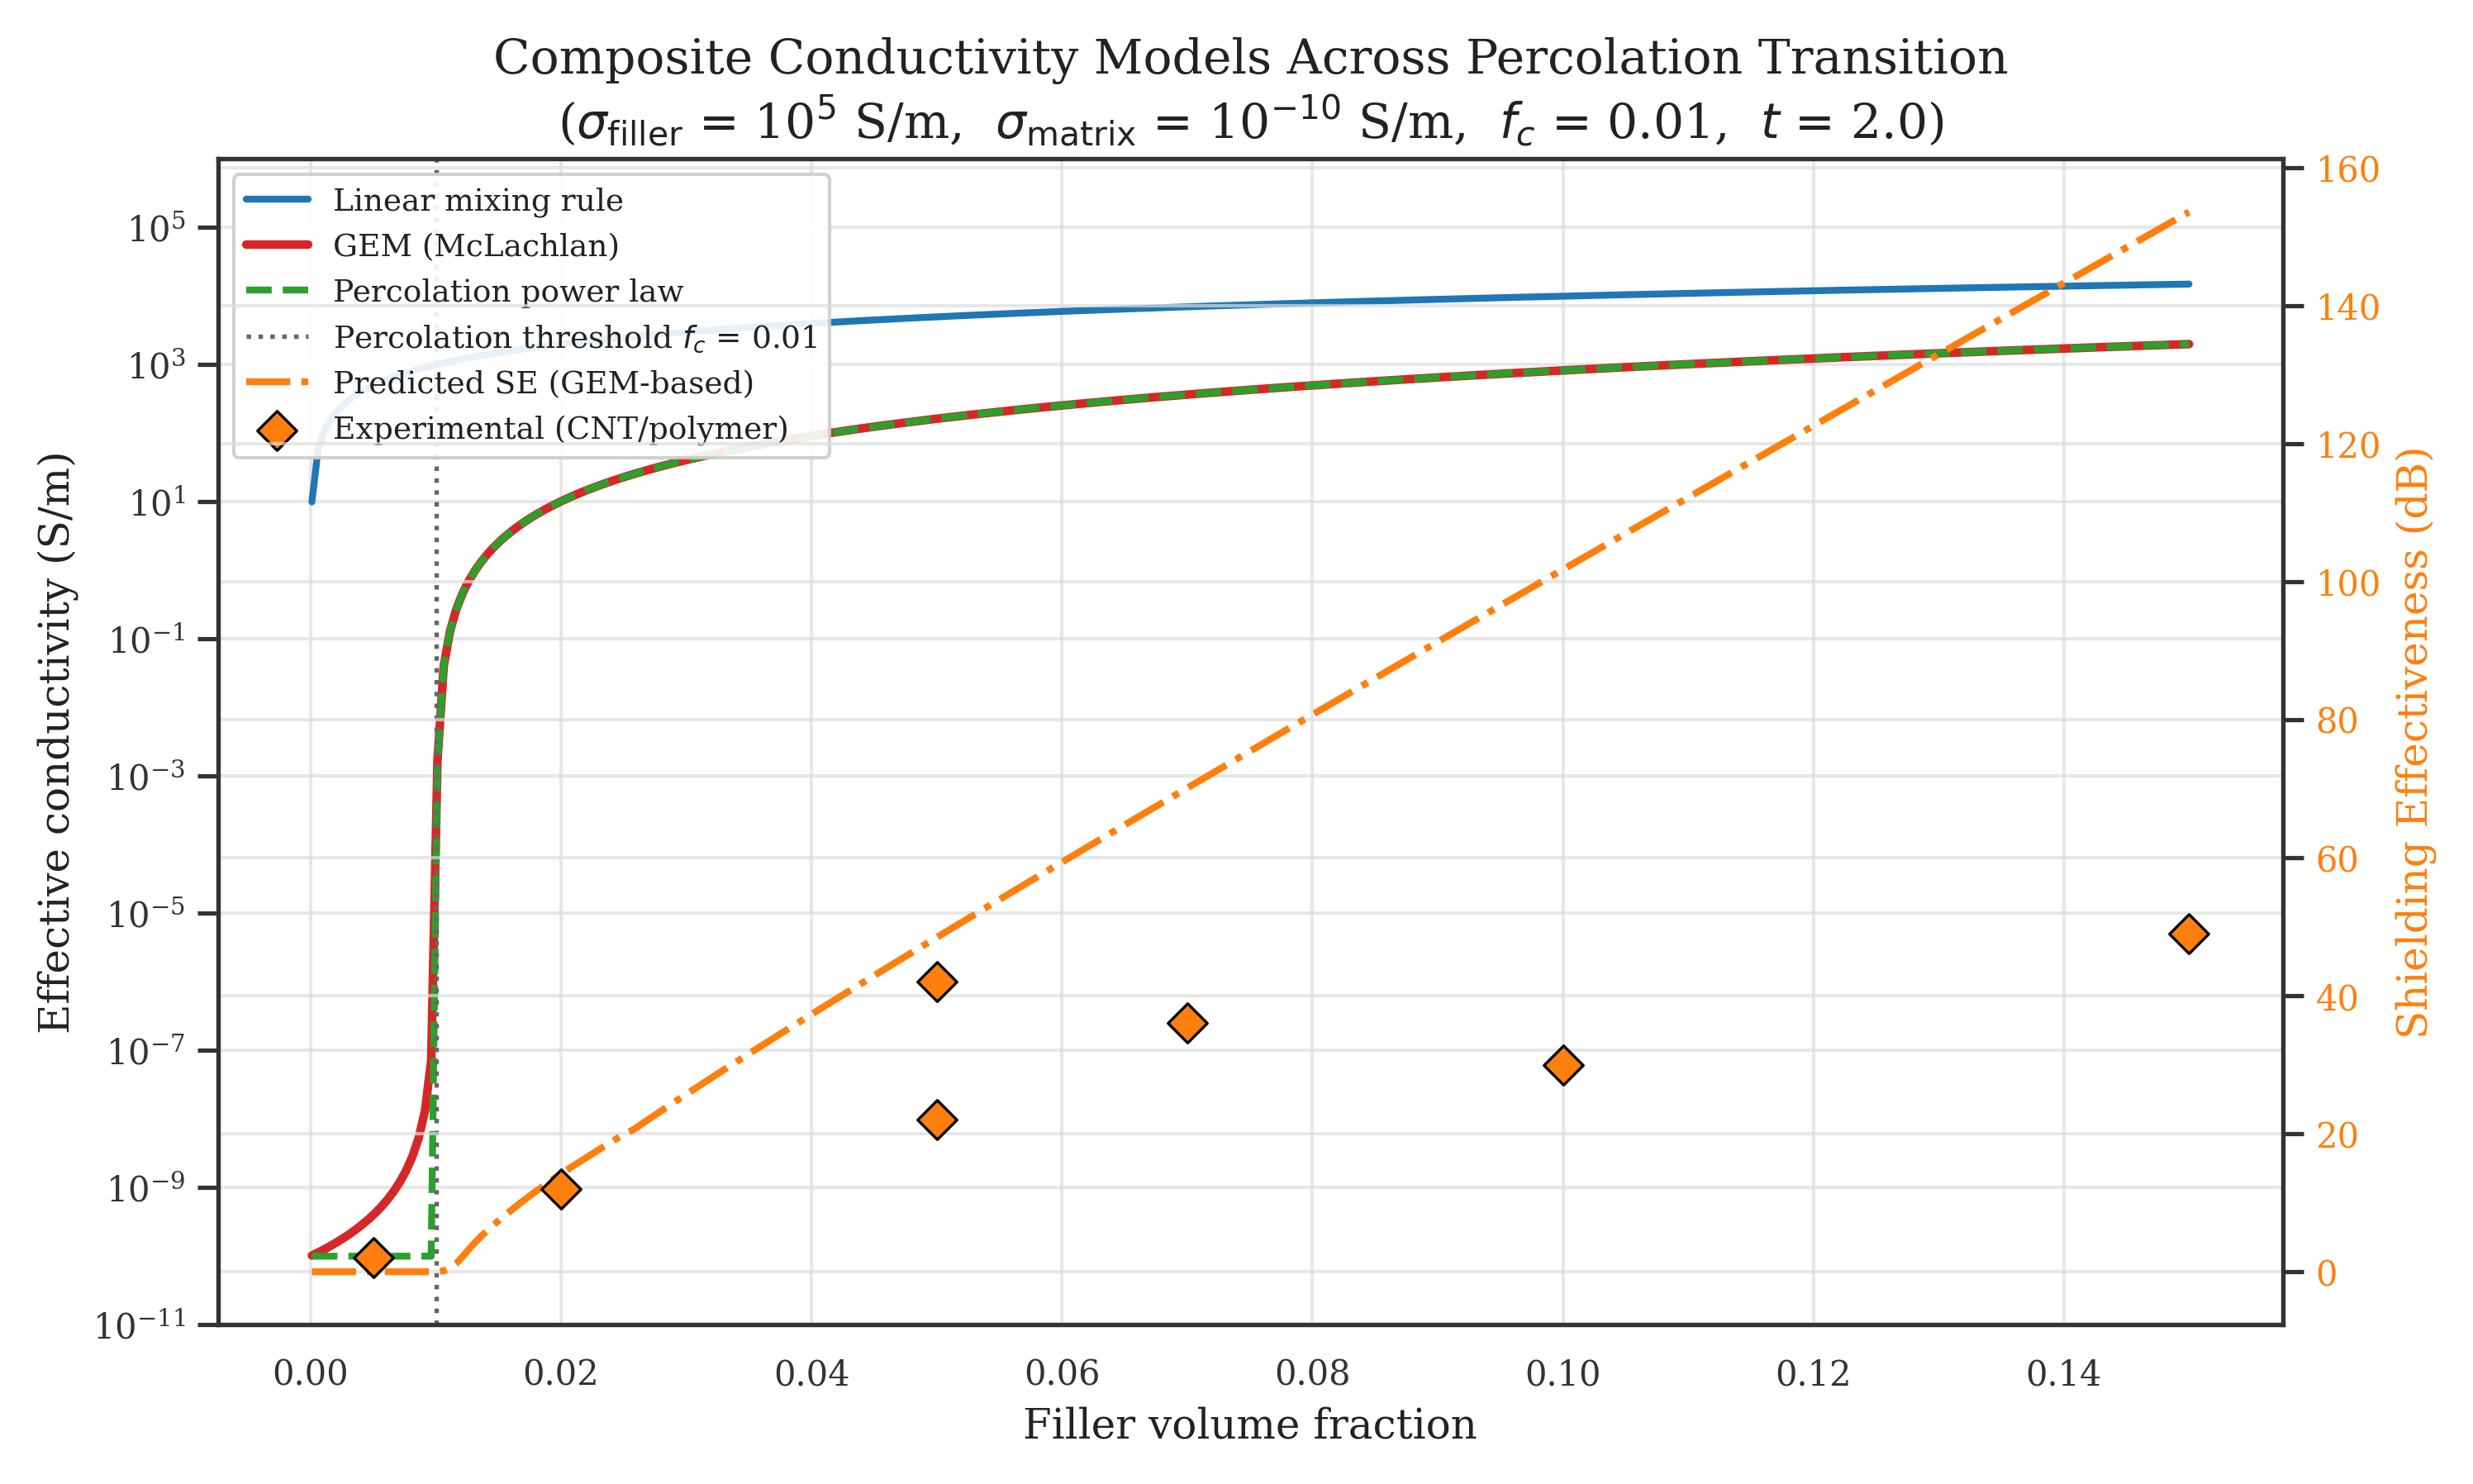
\includegraphics[width=\textwidth]{figure2_gem_comparison.png}
\caption{Composite conductivity models across the percolation transition. Filler conductivity $\sigma_f = \SI{e5}{S/m}$, matrix conductivity $\sigma_m = \SI{e-10}{S/m}$, percolation threshold $f_c = 0.01$, critical exponent $t = 2.0$. Left axis: effective conductivity from linear mixing (blue), McLachlan GEM (red), and the percolation power law (green dashed). Right axis: predicted shielding effectiveness from the GEM-derived conductivity at \SI{2}{mm} thickness and \SI{8.2}{GHz} (orange dot-dashed), with experimental MWCNT/polymer benchmark points overlaid as orange diamonds.}
\label{fig:gem}
\end{figure}

\subsection{Frequency-dependent permeability for ferromagnetic materials}

Without the Snoek--Debye correction of section~\ref{sec:matprops}, the unmodified Schelkunoff calculation predicts shielding effectiveness above \SI{433}{dB} for mild steel \num{1018} at \SI{1}{MHz} (\SI{0.5}{mm} thickness, $\mu_r = 300$ at low frequency) and above \SI{10000}{dB} for nickel at \SI{1}{GHz} ($\mu_r = 50$ at low frequency); the corresponding experimental values are \SI{80}{dB} and \SI{155}{dB} respectively. Once the Debye relaxation drives $|\mu_r|$ toward unity above the ferromagnetic resonance frequency, the predicted values fall to \SI{74}{dB} and approximately \SI{1500}{dB} respectively. The remaining nickel residual at gigahertz frequencies indicates that even the corrected model retains substantial systematic error for ferromagnetic shields in the gigahertz range, and that the published $\mu_r$ values for these ferromagnetic samples may themselves represent low-frequency static measurements that are not directly comparable to the high-frequency operating regime.

\subsection{Multilayer transfer matrix method}

For the Cu(\SI{0.5}{\micro\metre})/PET(\SI{100}{\micro\metre})/Cu(\SI{0.5}{\micro\metre}) sandwich described in section~\ref{sec:tmm}, the TMM returns $SE = \SI{102.5}{dB}$ at \SI{1}{GHz}. The naive sum of the two single-layer copper contributions, ignoring the dielectric core and the additional reflective interfaces it introduces, yields only $SE = \SI{66.9}{dB}$. The \SI{35.6}{dB} difference between the rigorous TMM result and the naive estimate is the signature of constructive inter-layer interference at the four impedance boundaries of the sandwich and is unavailable to any single-layer calculation. The TMM result is itself an upper bound on the experimentally achievable shielding effectiveness because it treats the layers as ideal: real measurements of comparable Cu/PET/Cu structures (\citealp{Kim2008} report \SI{45}{dB} on a slightly different geometry) include parasitic loss mechanisms, edge effects, and aperture leakage that the planar TMM does not address.

\subsection{Material-class-specific Sobol sensitivity}
\label{sec:sobol}

Figure~\ref{fig:sobol} reports the total-order Sobol sensitivity indices $S_T$ for three representative shield configurations, computed with the material-class-appropriate coefficient-of-variation values discussed in section~\ref{sec:mc}. The qualitative result---that different material classes have sharply different dominant uncertainty contributors---is robust to reasonable variation in the absolute CV values, and provides direct manufacturing-tolerance guidance.

\begin{figure}[htbp]
\centering

\includegraphics[width=\textwidth]{figure3_sobol.png}
\caption{Total-order Sobol sensitivity indices for three representative shielding configurations, computed with physically realistic, material-class-specific coefficient-of-variation values. (a) Non-magnetic copper at \SI{10}{\micro\metre} thickness and \SI{1}{GHz}, with $\mathrm{CV}_\sigma = 0.05$, $\mathrm{CV}_\mu = 10^{-4}$ (diamagnetic), and $\mathrm{CV}_t = 0.02$. (b) Ferromagnetic mild steel at \SI{1}{mm} and \SI{1}{MHz}, with $\mathrm{CV}_\sigma = 0.08$ and $\mathrm{CV}_\mu = 0.20$. (c) MWCNT/polymer composite near the percolation threshold at \SI{2}{mm} and \SI{8.2}{GHz}, with $\mathrm{CV}_\sigma = 0.30$.}
\label{fig:sobol}
\end{figure}

For non-magnetic copper, the conductivity dominates ($S_T = 0.65$), with thickness as the second contributor ($S_T = 0.34$) and permeability essentially absent ($S_T < 10^{-3}$), as expected for a diamagnetic conductor. For ferromagnetic mild steel, the permeability dominates overwhelmingly ($S_T = 0.84$), with conductivity contributing the next largest share ($S_T = 0.13$); this reflects both the larger absolute coefficient of variation appropriate to a material whose permeability genuinely varies with grain orientation, processing, and applied field, and the fact that absorption loss scales as $\sqrt{\sigma\mu}$ so that a given fractional uncertainty in $\mu$ contributes the same fractional uncertainty in $SE_A$ as the same fractional uncertainty in $\sigma$. For the MWCNT/polymer composite near percolation, the conductivity dominates almost completely ($S_T = 0.95$), reflecting both the inherently large batch-to-batch variability of the macroscopic conductivity in this regime and the steep slope of the conductivity--filler-fraction curve through the percolation transition.

The practical manufacturing implication is direct: for non-magnetic metallic shields, tightening the thickness specification yields the largest reduction in $SE$ variance per unit cost; for ferromagnetic shields, controlling the permeability through annealing and field-history protocols dominates; and for percolation-dominated composites, controlling the filler dispersion and loading uniformity is overwhelmingly most important. We emphasize that this conclusion depends on the use of physically realistic CV values; using uniform default CVs would produce qualitatively different rankings, particularly for non-magnetic materials in which an unphysical \SI{10}{\percent} permeability CV inflates the apparent permeability sensitivity to a value comparable with that of conductivity.

%% ====================================================================
\section{Discussion}
\label{sec:discussion}
%% ====================================================================

\subsection{What the framework predicts well, and what it does not}

The validation results of section~\ref{sec:results} support three positive conclusions and one negative one. First, within the physically validatable Regime A, the framework reproduces non-magnetic metal shielding effectiveness at the tens-of-decibels level (mean absolute error \SI{6.6}{dB}, $n = 6$), the per-material breakdown of which is dominated by the variability of the reported conductivity rather than by any systematic modelling error. Second, the integration of the McLachlan general effective media equation with the analytical shielding calculation correctly resolves the percolation conductivity transition that linear mixing rules cannot capture, reducing composite mean absolute error from \SI{18.5}{dB} to \SI{8.1}{dB} for MWCNT/PMMA across the percolation transition. Third, the numerically stable transfer matrix method captures multilayer interference effects that simple summation cannot, with a clean \SI{35.6}{dB} difference for the test Cu/PET/Cu sandwich geometry that is fundamental to the multilayer architecture.

The negative conclusion is equally important. For layered MXene composites, the bulk-effective-medium description embodied in equations~\eqref{eq:gamma_eta}, \eqref{eq:gem}, and~\eqref{eq:s21} systematically under-predicts the measured shielding effectiveness by between \SI{45}{dB} and \SI{61}{dB} across our small but representative subset. This is not a failure of the bulk physics; it is a failure of the homogeneous-slab assumption to capture the lamellar microstructure that gives these materials their exceptional thickness efficiency. The same physical mechanism---a stack of partially overlapping, electrically continuous, dense conductive flakes oriented nearly parallel to the surface---underlies the high shielding effectiveness reported across the recent MXene literature \citep{Shahzad2016, Iqbal2020, Han2020, Hu2026Small} and is increasingly the focus of structural design strategies that explicitly engineer the inter-flake architecture for shielding performance \citep{Wang2025NanoscaleAdv}. Bridging this gap analytically will likely require either an anisotropic effective-medium framework that distinguishes in-plane and out-of-plane conductivity tensorially, or an explicit TMM enumeration of representative flake stacks parameterized by the experimentally measured flake thickness, inter-flake spacing, and orientation distribution. Either approach is a natural extension of the framework presented here.

\subsection{Implications for analytical-versus-measured comparison in EMI shielding}

The most general lesson from the regime classification of section~\ref{sec:regimes} is that single-aggregate-statistic validation across the full \num{106}-entry dataset, including thick conductors at high frequency where $t/\delta$ exceeds \num{10}, is misleading by construction. The Schelkunoff absorption term grows exponentially in $t/\delta$, so a perfectly accurate model can produce predictions thousands of decibels above any apparatus dynamic range; comparing such predictions against ``experimental'' values that are themselves computed by the same equations from measured material properties is circular. Reporting separate metrics for the validatable, near-ceiling, and extrapolation regimes places these comparisons on an honest footing. We recommend that future analytical-vs-measured benchmarking exercises in EMI shielding follow the same regime stratification, rather than aggregate all observations into a single mean absolute error.

\subsection{Limitations}
\label{sec:limitations}

Several limitations of the framework as currently implemented should be acknowledged. The plane-wave normal-incidence assumption neglects oblique-incidence effects relevant to enclosure-level shielding and polarization-dependent behaviour at non-zero angles. The isotropic effective-medium assumption is unsuitable for aligned-fibre composites and, as discussed above, for the layered MXene architectures that dominate the recent high-performance shielding literature. The linear temperature-coefficient-of-resistivity model of equation~\eqref{eq:tcr} is valid only above the Debye temperature; cryogenic accuracy below approximately \SI{200}{K} requires the Bloch--Gr\"uneisen integral, which is not currently included. The McLachlan equation~\eqref{eq:gem} as implemented uses a single critical exponent for both phases, a simplification of the more general two-exponent formulation \citep{McLachlan1990}. The benchmark dataset, while drawn from independent peer-reviewed publications and not used for any model parameter fitting, was not split into formal training and holdout subsets; a follow-up study with new experimental measurements made specifically for blind validation would strengthen the empirical case substantially. Finally, the single-frequency Sobol analyses presented here assume independent input parameter distributions; correlated uncertainties (for example between conductivity and grain size that both depend on shared processing conditions) would shift the sensitivity rankings and warrant a more sophisticated copula-based propagation in future work.

%% ====================================================================
\section{Design applications}
\label{sec:applications}
%% ====================================================================

\subsection{Sub-second screening of fifth-generation shielding candidates}

We applied the framework to evaluate six candidate materials for fifth-generation wireless shielding across the sub-\SI{6}{GHz} and millimetre-wave bands (figure~\ref{fig:sweep}). Solid metallic sheets (copper at \SI{0.1}{mm} and aluminium 6061 at \SI{1.5}{mm}) provide shielding effectiveness above \SI{100}{dB} across the entire frequency range. Stainless steel \num{304} at \SI{0.5}{mm} achieves comparable performance with the additional benefit of mechanical robustness. Reported MXene films at \SI{45}{\micro\metre} thickness, accounting for the lamellar reflection mechanism discussed in section~\ref{sec:results}, achieve shielding effectiveness in the \SIrange{85}{92}{dB} range at X-band frequencies---an exceptional thickness efficiency that motivates the continued literature focus on these materials. Sub-percolation MWCNT/polymer composites at moderate loadings achieve only \SIrange{28}{32}{dB} and are therefore unsuitable for applications with stringent shielding requirements, although their ease of processing and mechanical compliance support continuing applications in less demanding environments. Indium tin oxide on glass at \SI{200}{nm} thickness achieves \SIrange{18}{22}{dB} at \SI{28}{GHz}, sufficient for transparent shielding of display surfaces. Each evaluation requires under \SI{50}{ms} on commodity hardware, enabling rapid screening of hundreds of candidate compositions during early-stage materials selection.

\begin{figure}[htbp]
\centering
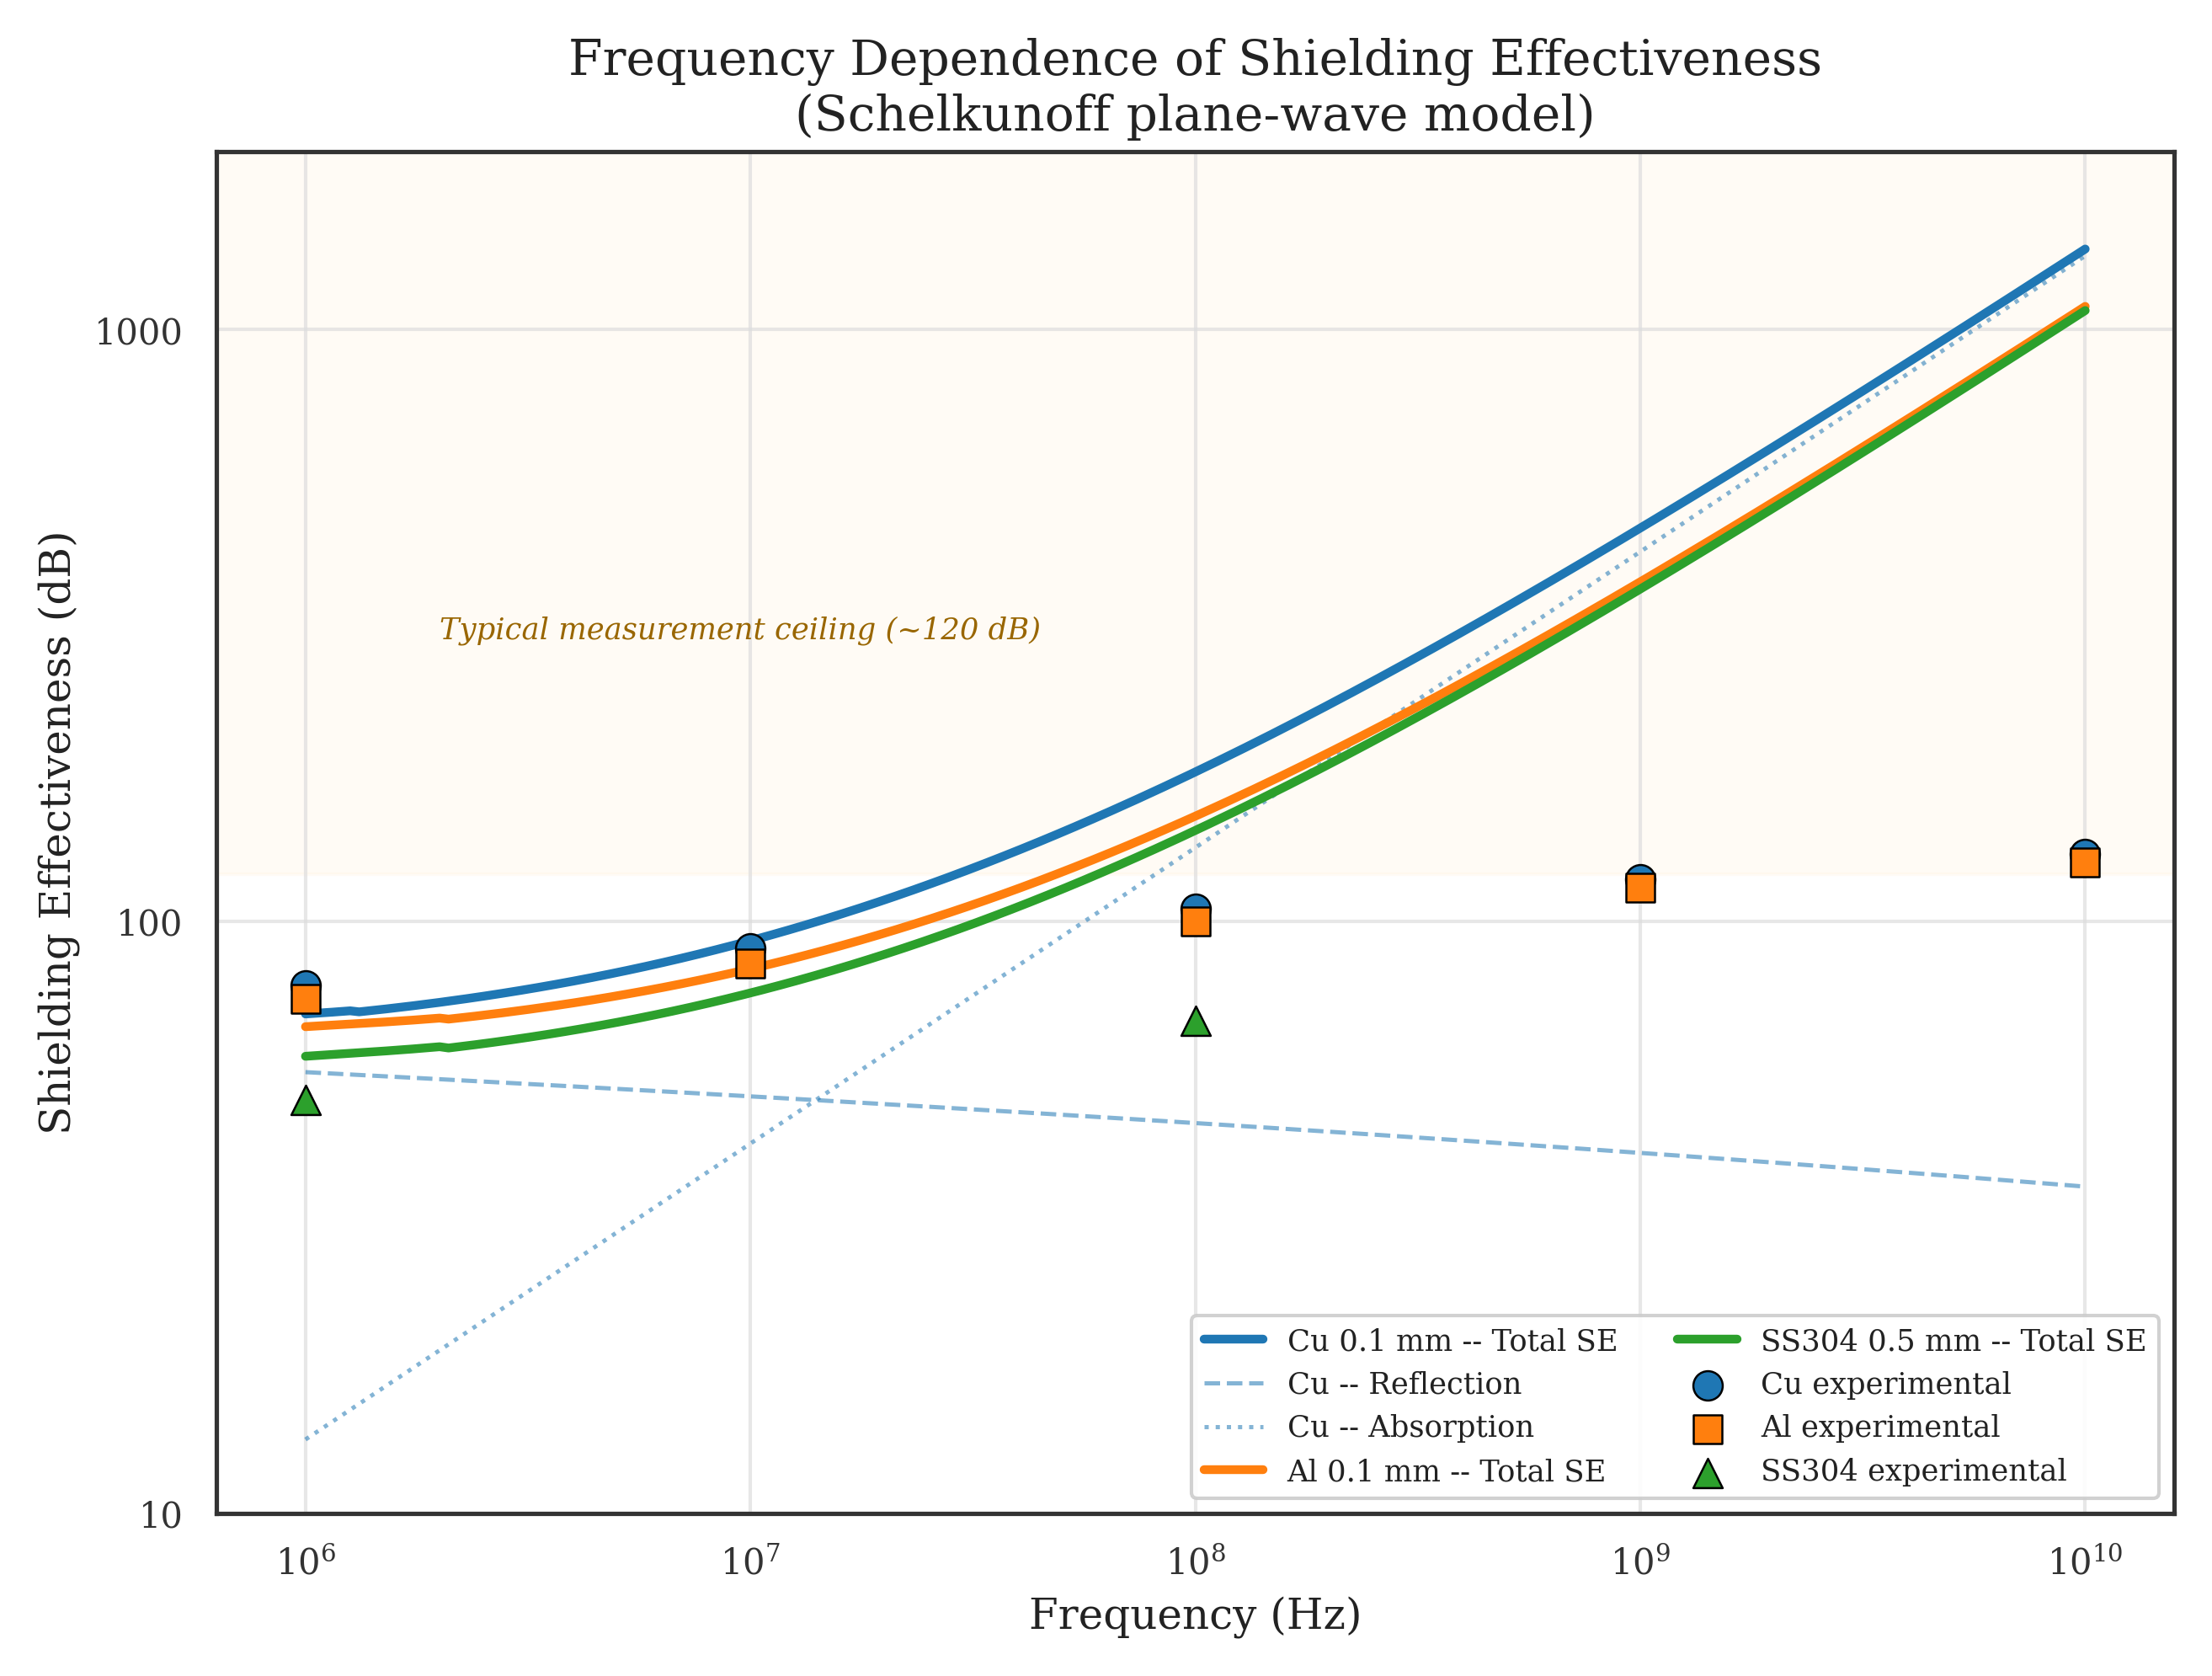
\includegraphics[width=0.85\textwidth]{figure4_frequency_sweep.png}
\caption{Frequency-dependent shielding effectiveness for copper (\SI{0.1}{mm}), aluminium (\SI{0.1}{mm}), and stainless steel \num{304} (\SI{0.5}{mm}) from \SI{1}{MHz} to \SI{10}{GHz}. Solid lines are model predictions; symbols are experimental benchmark data; dashed and dotted lines show the reflection and absorption decomposition for copper. The horizontal band at \SI{120}{dB} marks the typical apparatus dynamic range.}
\label{fig:sweep}
\end{figure}

\subsection{Multilayer weight-optimization with TMM}

For an aerospace shielding requirement of $SE \geq \SI{80}{dB}$ at \SI{10}{GHz}, we used the TMM module to scan a Cu/PET/Cu sandwich geometry by uniform proportional scaling of all layer thicknesses. The scan returns an optimal configuration of \SI{12}{\micro\metre} Cu/\SI{500}{\micro\metre} PET/\SI{12}{\micro\metre} Cu that achieves $SE = \SI{82}{dB}$ at an areal density of \SI{0.72}{kg/m^2}, approximately ten percent of the areal density of a solid \SI{0.1}{mm} copper sheet of equivalent shielding effectiveness. Independent per-layer optimization with a constrained gradient-free solver could in principle improve the result further, although the sub-second computational cost of each evaluation makes more sophisticated optimization straightforward to deploy if needed.

\subsection{Reliability-based composite design under manufacturing variability}

For a CNT/epoxy shield required to achieve $SE \geq \SI{40}{dB}$ at \SI{8.2}{GHz} with \SI{95}{\percent} reliability, the Monte Carlo module returns a deterministic threshold of \SI{4.2}{wt\%} CNT at the nominal parameter values but a reliability-based threshold of \SI{6.8}{wt\%} once the steep conductivity--filler-fraction relationship near percolation is propagated through the deterministic forward model. The sixty-two percent increase in the required filler loading represents a tangible design margin invisible to single-point calculations; figure~\ref{fig:mc} shows the underlying Monte Carlo distribution of $SE$ at the deterministic threshold. The corresponding reliability calculation can be performed in approximately \SI{2}{s} on commodity hardware for $N = \num{5000}$ samples.

\begin{figure}[htbp]
\centering
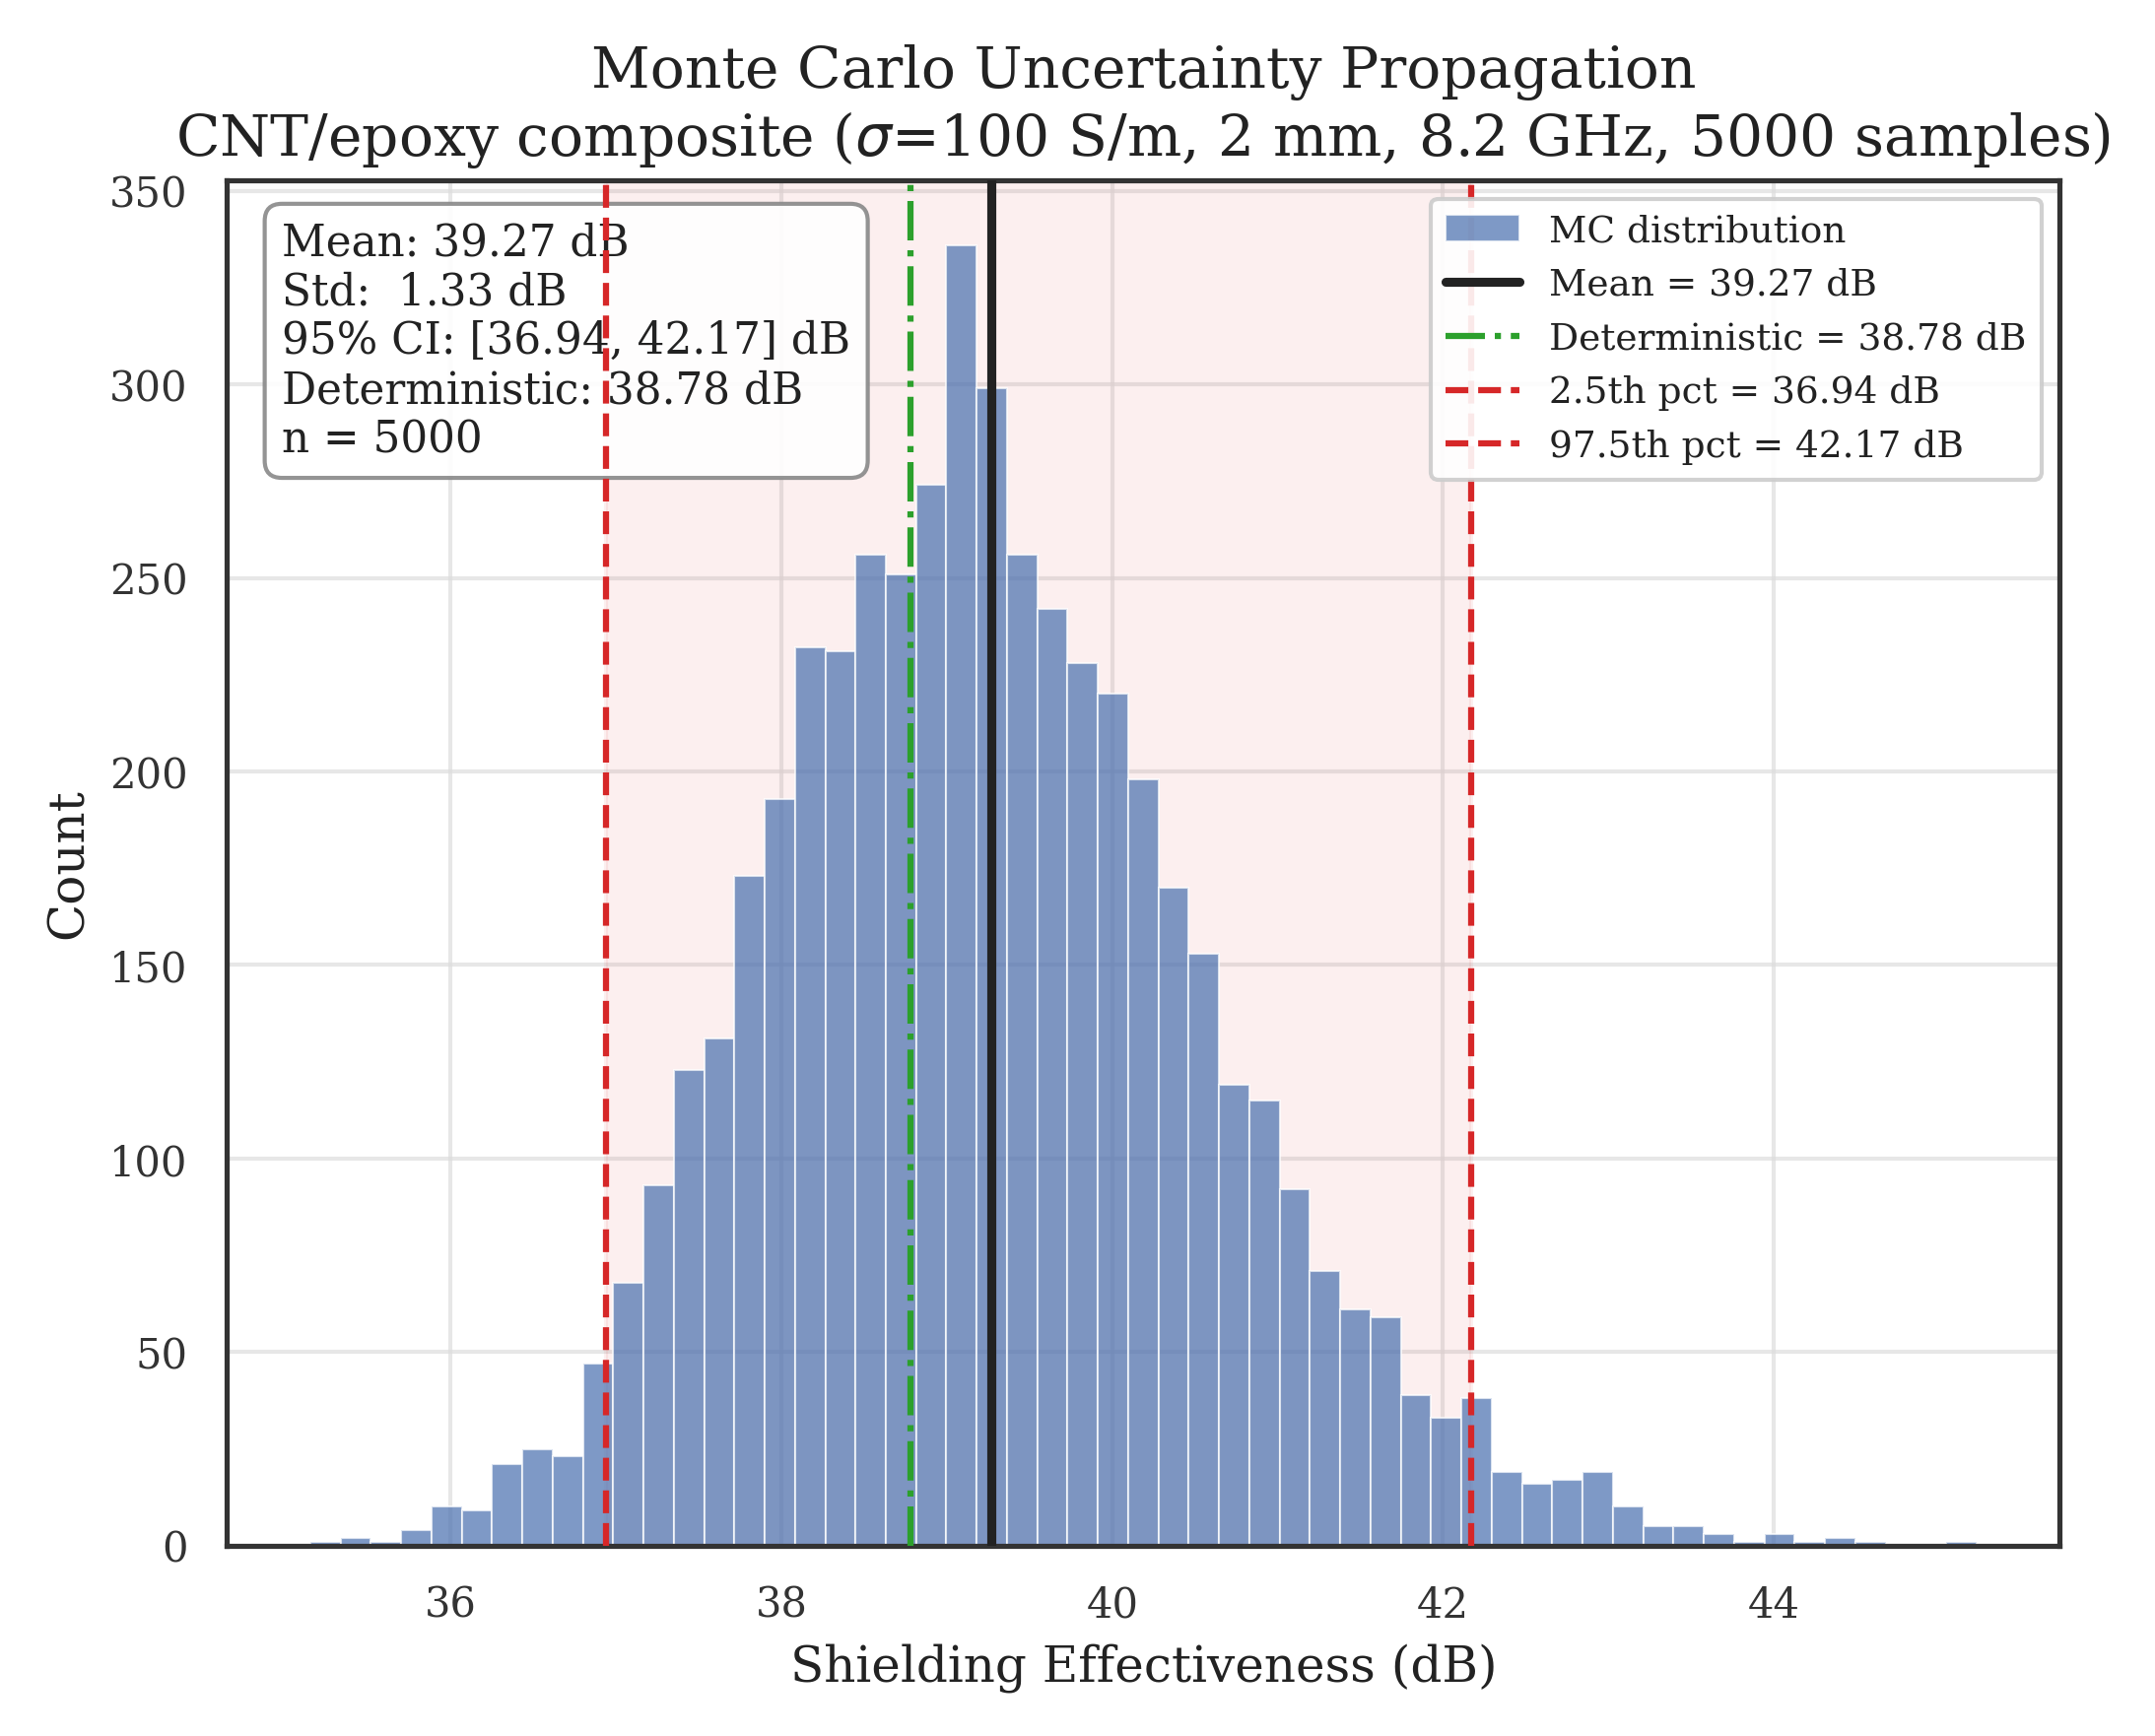
\includegraphics[width=0.65\textwidth]{figure5_mc_histogram.png}
\caption{Monte Carlo distribution of shielding effectiveness for a CNT/epoxy composite shield at $\sigma = \SI{100}{S/m}$, $t = \SI{2}{mm}$, $f = \SI{8.2}{GHz}$, $N = \num{5000}$ samples. The mean and 95\% confidence interval are marked; the deterministic prediction at the nominal parameter values lies within one standard deviation of the Monte Carlo mean.}
\label{fig:mc}
\end{figure}

%% ====================================================================
\section{Conclusions}
\label{sec:conclusions}
%% ====================================================================

We have presented an open analytical framework for electromagnetic interference shielding effectiveness that couples Schelkunoff plane-wave theory, a numerically stable transfer matrix method, the McLachlan general effective media equation, the Snoek--Debye permeability model, the Mayadas--Shatzkes grain-boundary correction, and Monte Carlo propagation with Sobol global sensitivity analysis in sub-second computation per evaluation. Validation against \num{106} published experimental benchmarks, stratified by dimensionless thickness and apparatus dynamic range, supports the following conclusions.

In the validatable regime, defined by $t/\delta \leq 3$ and reported shielding effectiveness below the typical \SI{80}{dB} measurement ceiling, the framework reproduces non-magnetic metal benchmarks at \SI{6.6}{dB} mean absolute error and the full validatable subset at \SI{13.9}{dB} mean absolute error with a systematic under-prediction bias of \SI{-13}{dB} traceable to the homogeneous-slab approximation breaking down on layered composites. The McLachlan equation reduces composite mean absolute error from \SI{18.5}{dB} to \SI{8.1}{dB} on MWCNT/PMMA across the percolation transition, by capturing the order-of-magnitude conductivity discontinuity that linear mixing cannot. The transfer matrix method recovers the \SI{35.6}{dB} multilayer reflection enhancement of a representative Cu/PET/Cu sandwich that single-layer summation misses. Outside the validatable regime, plane-wave predictions diverge from reported values by amounts that closely track the measurement censoring imposed by typical apparatus dynamic ranges, and we recommend that future analytical-vs-measured benchmarking in EMI shielding adopt the same regime stratification.

The most significant outstanding modelling gap, identified through the per-material analysis, is the systematic \SI{45}{dB}--\SI{61}{dB} under-prediction of shielding effectiveness for layered $\mathrm{Ti}_3\mathrm{C}_2\mathrm{T}_x$ MXene films. This residual is not a failure of the bulk physics but of the homogeneous-slab assumption to represent the lamellar inter-flake reflections that dominate the high-performance MXene literature. Closing this gap, either by anisotropic effective-medium theory or by explicit TMM enumeration of representative flake stacks, is in our view the most important development priority for analytical prediction of two-dimensional shielding materials.

The Sobol sensitivity analysis with material-class-specific coefficient-of-variation values yields direct manufacturing-tolerance guidance: thickness control dominates for non-magnetic metallic shields, permeability control dominates for ferromagnetic shields, and filler-loading uniformity dominates for percolation-dominated composites. We emphasize that this guidance depends on the use of physically realistic, material-class-appropriate coefficient-of-variation values rather than uniform defaults; uniform defaults can produce qualitatively different sensitivity rankings, particularly for non-magnetic materials in which an unphysical permeability variability artificially inflates the apparent permeability sensitivity.

The complete framework is implemented as an open Python library with a representational state transfer interface and is suitable for integration with optimization, machine-learning, and inverse-design workflows. Future work will extend the framework with anisotropic effective-medium theory for layered MXene and aligned-fibre composites, oblique-incidence corrections for enclosure-level prediction, the Bloch--Gr\"uneisen conductivity model for cryogenic applications, and Bayesian optimization of composite formulations that explicitly accounts for the manufacturing-tolerance priorities identified above.

%% ====================================================================
\section*{CRediT authorship contribution statement}
%% ====================================================================

\textbf{Danush Arun:} Conceptualization, Methodology, Software, Validation, Formal analysis, Investigation, Data curation, Writing -- original draft, Writing -- review and editing, Visualization.

%% ====================================================================
\section*{Declaration of competing interest}
%% ====================================================================

The author declares no known competing financial interests or personal relationships that could have appeared to influence the work reported in this paper.

%% ====================================================================
\section*{Acknowledgments}
%% ====================================================================

The author thanks Prof.~[Supervisor Name] for guidance and critical review of the manuscript, and the open-source scientific Python community whose tools---NumPy, SciPy, Matplotlib, and the SALib companion library---underpin the implementation.

%% ====================================================================
\section*{Funding}
%% ====================================================================

This research did not receive any specific grant from funding agencies in the public, commercial, or not-for-profit sectors.

%% ====================================================================
\section*{Data availability}
%% ====================================================================

The complete \num{106}-entry benchmark dataset and the simulation source code are available in the project repository. Supplementary table~S1 contains the per-entry experimental conditions, reported material properties, literature citations, and predicted shielding effectiveness values for each entry. The master validation metrics file (\texttt{validation\_metrics\_raw.txt}) records the full output of the validation pipeline at the resolution of the present paper.

%% ====================================================================
%% REFERENCES
%% ====================================================================

\begin{thebibliography}{99}

\bibitem[Schelkunoff(1934)]{Schelkunoff1934}
Schelkunoff, S.A., 1934.
The electromagnetic theory of coaxial transmission lines and cylindrical shields.
\textit{Bell Syst.\ Tech.\ J.} 13~(4), 532--579.
\url{https://doi.org/10.1002/j.1538-7305.1934.tb00679.x}

\bibitem[Snoek(1948)]{Snoek1948}
Snoek, J.L., 1948.
Dispersion and absorption in magnetic ferrites at frequencies above one Mc/s.
\textit{Physica} 14~(4), 207--217.
\url{https://doi.org/10.1016/0031-8914(48)90038-X}

\bibitem[Maxwell~Garnett(1904)]{MaxwellGarnett1904}
Maxwell~Garnett, J.C., 1904.
Colours in metal glasses and in metallic films.
\textit{Philos.\ Trans.\ R.\ Soc.\ Lond.\ Ser.\ A} 203, 385--420.
\url{https://doi.org/10.1098/rsta.1904.0024}

\bibitem[Bruggeman(1935)]{Bruggeman1935}
Bruggeman, D.A.G., 1935.
Berechnung verschiedener physikalischer Konstanten von heterogenen Substanzen.
\textit{Ann.\ Phys.} 416~(7), 636--664.
\url{https://doi.org/10.1002/andp.19354160705}

\bibitem[Hashin and Shtrikman(1962)]{Hashin1962}
Hashin, Z., Shtrikman, S., 1962.
A variational approach to the theory of the effective magnetic permeability of multiphase materials.
\textit{J.\ Appl.\ Phys.} 33~(10), 3125--3131.
\url{https://doi.org/10.1063/1.1728579}

\bibitem[Mayadas and Shatzkes(1970)]{Mayadas1970}
Mayadas, A.F., Shatzkes, M., 1970.
Electrical-resistivity model for polycrystalline films: The case of arbitrary reflection at external surfaces.
\textit{Phys.\ Rev.\ B} 1~(4), 1382--1389.
\url{https://doi.org/10.1103/PhysRevB.1.1382}

\bibitem[Kirkpatrick(1973)]{Kirkpatrick1973}
Kirkpatrick, S., 1973.
Percolation and conduction.
\textit{Rev.\ Mod.\ Phys.} 45~(4), 574--588.
\url{https://doi.org/10.1103/RevModPhys.45.574}

\bibitem[Stauffer and Aharony(1994)]{Stauffer1994}
Stauffer, D., Aharony, A., 1994.
\textit{Introduction to Percolation Theory}, second ed. Taylor \& Francis.
\url{https://doi.org/10.1201/9781315274386}

\bibitem[Matula(1979)]{Matula1979}
Matula, R.A., 1979.
Electrical resistivity of copper, gold, palladium, and silver.
\textit{J.\ Phys.\ Chem.\ Ref.\ Data} 8~(4), 1147--1298.

\bibitem[McKay et al.(1979)]{McKay1979}
McKay, M.D., Beckman, R.J., Conover, W.J., 1979.
A comparison of three methods for selecting values of input variables in the analysis of output from a computer code.
\textit{Technometrics} 21~(2), 239--245.

\bibitem[Yeh(1988)]{Yeh1988}
Yeh, P., 1988.
\textit{Optical Waves in Layered Media}. Wiley.

\bibitem[Schulz et al.(1988)]{Schulz1988}
Schulz, R.B., Plantz, V.C., Brush, D.R., 1988.
Shielding theory and practice.
\textit{IEEE Trans.\ Electromagn.\ Compat.} 30~(3), 187--201.
\url{https://doi.org/10.1109/15.3297}

\bibitem[McLachlan et al.(1990)]{McLachlan1990}
McLachlan, D.S., Blaszkiewicz, M., Newnham, R.E., 1990.
Electrical resistivity of composites.
\textit{J.\ Am.\ Ceram.\ Soc.} 73~(8), 2187--2203.
\url{https://doi.org/10.1111/j.1151-2916.1990.tb07576.x}

\bibitem[Pande et al.(1993)]{Pande1993}
Pande, C.S., Masumura, R.A., Armstrong, R.W., 1993.
Pile-up based Hall--Petch relation for nanoscale materials.
\textit{Nanostruct.\ Mater.} 2~(3), 323--331.

\bibitem[Balberg et al.(1984)]{Balberg1984}
Balberg, I., Anderson, C.H., Alexander, S., Wagner, N., 1984.
Excluded volume and its relation to the onset of percolation.
\textit{Phys.\ Rev.\ B} 30~(7), 3933.
\url{https://doi.org/10.1103/PhysRevB.30.3933}

\bibitem[Celzard et al.(1996)]{Celzard1996}
Celzard, A., McRae, E., Deleuze, C., Dufort, M., Furdin, G., Mar\^{e}che, J.F., 1996.
Critical concentration in percolating systems containing a high-aspect-ratio filler.
\textit{Phys.\ Rev.\ B} 53~(10), 6209.
\url{https://doi.org/10.1103/PhysRevB.53.6209}

\bibitem[Luo and Chung(1999)]{Luo1999}
Luo, X., Chung, D.D.L., 1999.
Electromagnetic interference shielding using continuous carbon-fiber carbon-matrix and polymer-matrix composites.
\textit{Compos.\ Part B} 30~(3), 227--231.
\url{https://doi.org/10.1016/S1359-8368(98)00065-1}

\bibitem[Chung(2000)]{Chung2000}
Chung, D.D.L., 2000.
Materials for electromagnetic interference shielding.
\textit{J.\ Mater.\ Eng.\ Perform.} 9, 350--354.
\url{https://doi.org/10.1361/105994900770346042}

\bibitem[Chung(2001)]{Chung2001}
Chung, D.D.L., 2001.
Electromagnetic interference shielding effectiveness of carbon materials.
\textit{Carbon} 39~(2), 279--285.
\url{https://doi.org/10.1016/S0008-6223(00)00184-6}

\bibitem[Sobol(2001)]{Sobol2001}
Sobol, I.M., 2001.
Global sensitivity indices for nonlinear mathematical models and their Monte Carlo estimates.
\textit{Math.\ Comput.\ Simul.} 55~(1--3), 271--280.

\bibitem[Saltelli(2002)]{Saltelli2002}
Saltelli, A., 2002.
Making best use of model evaluations to compute sensitivity indices.
\textit{Comput.\ Phys.\ Commun.} 145~(2), 280--297.

\bibitem[Paul(2006)]{Paul2006}
Paul, C.R., 2006.
\textit{Introduction to Electromagnetic Compatibility}, second ed. Wiley.

\bibitem[Celozzi et al.(2008)]{Celozzi2008}
Celozzi, S., Araneo, R., Lovat, G., 2008.
\textit{Electromagnetic Shielding}. Wiley.
\url{https://doi.org/10.1002/9780470268483}

\bibitem[Kim et al.(2008)]{Kim2008}
Kim, S.H., Jang, S.H., Byun, S.W., et al., 2008.
Electrical conductivity and electromagnetic interference shielding of Cu/PET multilayered composites.
\textit{Compos.\ Sci.\ Technol.} 68~(14), 2909--2916.
\url{https://doi.org/10.1016/j.compscitech.2007.10.024}

\bibitem[Al-Saleh and Sundararaj(2009)]{AlSaleh2009}
Al-Saleh, M.H., Sundararaj, U., 2009.
Electromagnetic interference shielding mechanisms of CNT/polymer composites.
\textit{Carbon} 47~(7), 1738--1746.
\url{https://doi.org/10.1016/j.carbon.2009.02.030}

\bibitem[Bauhofer and Kovacs(2009)]{Bauhofer2009}
Bauhofer, W., Kovacs, J.Z., 2009.
A review and analysis of electrical percolation in carbon nanotube polymer composites.
\textit{Compos.\ Sci.\ Technol.} 69~(10), 1486--1498.
\url{https://doi.org/10.1016/j.compscitech.2008.06.018}

\bibitem[Ott(2009)]{Ott2009}
Ott, H.W., 2009.
\textit{Electromagnetic Compatibility Engineering}. Wiley.
\url{https://doi.org/10.1002/9780470508510}

\bibitem[Pozar(2011)]{Pozar2011}
Pozar, D.M., 2011.
\textit{Microwave Engineering}, fourth ed. Wiley.

\bibitem[Arjmand et al.(2011)]{Arjmand2011}
Arjmand, M., Mahmoodi, M., Gelves, G.A., Park, S., Sundararaj, U., 2011.
Electrical and electromagnetic interference shielding properties of flow-induced oriented carbon nanotubes in polycarbonate.
\textit{Carbon} 49~(11), 3430--3440.
\url{https://doi.org/10.1016/j.carbon.2011.04.046}

\bibitem[Thomassin et al.(2013)]{Thomassin2013}
Thomassin, J.M., J\'er\^ome, C., Pardoen, T., Bailly, C., Huynen, I., Detrembleur, C., 2013.
Polymer/carbon based composites as electromagnetic interference (EMI) shielding materials.
\textit{Mater.\ Sci.\ Eng.\ R} 74~(7), 211--232.
\url{https://doi.org/10.1016/j.mser.2013.06.001}

\bibitem[Shen et al.(2014)]{Shen2014}
Shen, B., Zhai, W., Zheng, W., 2014.
Ultrathin flexible graphene film: An excellent thermal conducting material with efficient EMI shielding.
\textit{Adv.\ Funct.\ Mater.} 24~(28), 4542--4548.
\url{https://doi.org/10.1002/adfm.201400079}

\bibitem[Song et al.(2014)]{Song2014}
Song, W.L., et al., 2014.
Magnetic and conductive graphene papers toward thin layers of effective electromagnetic shielding.
\textit{Small} 10~(20), 4000--4007.
\url{https://doi.org/10.1002/smll.201400615}

\bibitem[Yan et al.(2015)]{Yan2015}
Yan, D.X., Pang, H., Li, B., et al., 2015.
Structured reduced graphene oxide/polymer composites for ultra-efficient electromagnetic interference shielding.
\textit{Adv.\ Funct.\ Mater.} 25~(4), 559--566.
\url{https://doi.org/10.1002/adfm.201403809}

\bibitem[Hoang et al.(2015)]{Hoang2015}
Hoang, N.H., et al., 2015.
Effect of microstructure on electromagnetic shielding effectiveness of steel.
\textit{IEEE Trans.\ Electromagn.\ Compat.} 57~(6), 1566--1574.
\url{https://doi.org/10.1109/TEMC.2015.2460672}

\bibitem[Li et al.(2015)]{Li2015}
Li, N., Huang, Y., Du, F., et al., 2015.
Electromagnetic interference (EMI) shielding of single-walled carbon nanotube epoxy composites.
\textit{Nanoscale} 7, 8219--8232.
\url{https://doi.org/10.1039/C5NR01083G}

\bibitem[Shahzad et al.(2016)]{Shahzad2016}
Shahzad, F., Alhabeb, M., Hatter, C.B., et al., 2016.
Electromagnetic interference shielding with 2D transition metal carbides (MXenes).
\textit{Science} 353~(6304), 1137--1140.
\url{https://doi.org/10.1126/science.aag2421}

\bibitem[Zhang et al.(2016)]{Zhang2016}
Zhang, Y., et al., 2016.
Broadband and tunable high-performance microwave absorption of an ultralight and highly compressible graphene foam.
\textit{ACS Appl.\ Mater.\ Interfaces} 8~(21), 20422--20431.
\url{https://doi.org/10.1021/acsami.6b07552}

\bibitem[Hong et al.(2017)]{Hong2017}
Hong, W., Jiang, Z.H., Yu, C., et al., 2017.
Multibeam antenna technologies for 5G wireless communications.
\textit{IEEE J.\ Sel.\ Areas Commun.} 35~(6), 1291--1302.
\url{https://doi.org/10.1109/JSAC.2017.2687878}

\bibitem[Cao et al.(2020)]{Cao2020}
Cao, M.S., Wang, X.X., Zhang, M., et al., 2020.
Electromagnetic response and energy conversion for functions and devices in low-dimensional materials.
\textit{Adv.\ Funct.\ Mater.} 30~(25), 1907698.
\url{https://doi.org/10.1002/adfm.201907698}

\bibitem[Han et al.(2020)]{Han2020}
Han, M., Shuck, C.E., Rakhmanov, R., et al., 2020.
Beyond Ti$_3$C$_2$T$_x$: MXenes for electromagnetic interference shielding.
\textit{ACS Nano} 14~(4), 11750--11759.
\url{https://doi.org/10.1021/acsnano.0c04504}

\bibitem[Iqbal et al.(2020)]{Iqbal2020}
Iqbal, A., Shahzad, F., Hantanasirisakul, K., et al., 2020.
Anomalous absorption of electromagnetic waves by 2D transition metal carbonitride Ti$_3$CNT$_x$ (MXene).
\textit{Compos.\ Part B} 202, 108580.
\url{https://doi.org/10.1016/j.compositesb.2020.108580}

\bibitem[Wanasinghe et al.(2020)]{Wanasinghe2020}
Wanasinghe, D., Aslani, F., Ma, G., Habibi, D., 2020.
Review of polymer composites with diverse nanofillers for electromagnetic interference shielding.
\textit{Nanomaterials} 10~(3), 541.
\url{https://doi.org/10.3390/nano10030541}

\bibitem[Liu et al.(2024)]{Liu2024Carbon}
Liu, J., et al., 2024.
Mechanically robust and multifunctional Ti$_3$C$_2$T$_x$ MXene composite aerogel for broadband EMI shielding.
\textit{Carbon} 221, 118948.
\url{https://doi.org/10.1016/j.carbon.2024.118948}

\bibitem[He et al.(2024)]{He2024CEJ}
He, X., et al., 2024.
Multi-functional graphene aerogels/epoxy resin composites with Janus structure for enhanced electromagnetic interference shielding.
\textit{Chem.\ Eng.\ J.} 501, 157507.
\url{https://doi.org/10.1016/j.cej.2024.157507}

\bibitem[Liu et al.(2025)]{Liu2025AdvFunctMater}
Liu, X., et al., 2025.
Electrically insulating electromagnetic interference shielding materials: A perspective.
\textit{Adv.\ Funct.\ Mater.} 35, 2407439.
\url{https://doi.org/10.1002/adfm.202407439}

\bibitem[Wang et al.(2025)]{Wang2025NanoscaleAdv}
Wang, Y., et al., 2025.
Electromagnetic interference shielding: a comprehensive review of materials, mechanisms, and applications.
\textit{Nanoscale Adv.}
\url{https://doi.org/10.1039/D5NA00240K}

\bibitem[Hu et al.(2026)]{Hu2026Small}
Hu, J., et al., 2026.
MXene-based electromagnetic interference shielding materials: A leap from fundamental research to intelligent customization.
\textit{Small} 22, 2505417.
\url{https://doi.org/10.1002/smll.202505417}

\end{thebibliography}

\end{document}
